\documentclass [PhD] {uclathes}

% \input {mymacros}                         % personal LaTeX macros

%%%%%%%%%%%%%%%%%%%%%%%%%%%%%%%%%%%%%%%%%%%%%%%%%%%%%%%%%%%%%%%%%%%%%%
%
% Usually things live in separate flies.
%
 \input {preamble}                           % preliminary page info

%%%%%%%%%%%%%%%%%%%%%%%%%%%%%%%%%%%%%%%%%%%%%%%%%%%%%%%%%%%%%%%%%%%%%%%%
%                                                                      %
%                          PRELIMINARY PAGES                           %
%                                                                      %
%%%%%%%%%%%%%%%%%%%%%%%%%%%%%%%%%%%%%%%%%%%%%%%%%%%%%%%%%%%%%%%%%%%%%%%%

\title          {Knowledge of the Social Sciences}
\author         {Brooks Ambrose}
% Note: department is really your area of research.  I.e. leave out 'Department of'.
\department     {Sociology}
% Note:  degreeyear should be optional, but as of  5-Feb-96
% it seems required or you get a year of ``2''.   -johnh
\degreeyear     {2019}

%%%%%%%%%%%%%%%%%%%%%%%%%%%%%%%%%%%%%%%%%%%%%%%%%%%%%%%%%%%%%%%%%%%%%%%%

\member         {Gabriel Rossman}
\member         {Jacob Foster}
\member         {Barbara Lawrence}
\chair          {Lynne G. Zucker}
%\chair          {Chair's name 2}
%\chair          {Chair's name 3}

%%%%%%%%%%%%%%%%%%%%%%%%%%%%%%%%%%%%%%%%%%%%%%%%%%%%%%%%%%%%%%%%%%%%%%%%

\dedication     {\textsl{To Adena \ldots \\
                my mound builder,
                that you may learn to care
                about who came before
                and who will come after. \\~\\
                To Bill the theorist, \\
                Jean the historian, and \\
                Julia the artist \ldots \\
                I am nothing more \\
                than each of you \\~\\
                To Jessica \ldots \\
                I shall never grow so old again! \\
                (I promise)
                }}

%%%%%%%%%%%%%%%%%%%%%%%%%%%%%%%%%%%%%%%%%%%%%%%%%%%%%%%%%%%%%%%%%%%%%%%%

\acknowledgments {
I would like to acknowledge the years of support I have received from many wonderful people. First and foremost I would like to thank my family for supporting my education for just one more decade than they expected. I am happy that you will finally know what I was doing.

Professor Mark Gould of Haverford College introduced me to sociology and helped me feel connected to something much older and bigger than myself. He together with Victor Lidz showed me the importance of a theoretical imagination in the study of history. Any creativity in my use of data is attributable to their creativity in the use of ideas.

Lynne Zucker has been a mentor and a friend. She demonstrates that great intelligence and great kindness take one farther than either could alone. I would not have finished without the courage she inspired. I am honored to share co-authorship of Chapter 4 of this manuscript with her. Her knowledge of data sources and the importance of economic history, as well as her leadership in institutional and organizational theory, helped to turn an interesting project into an important one.

Jacob Foster, Barbara Lawrence, and Gabriel Rossman have provided years of support and guidance. I am eternally grateful for their tireless dedication to their students.

I have the deepest faith in Johann Koehler and know that he will do great things. I will always trust him to care deeply about me and my work.

Peter Norlander invited me to apply for my first faculty position at the University of California, and opened up a new world of opportunities for me as a result.

The colleagues and friends I have met through the D-Lab at the University of California are the source of my fascination with machine reading of texts and my capacity to do something about it. My fellow travelers in the D-Lab Computational Text Analysis Working Group introduced me to most of the methods I use in this manuscript. Without the lessons I learned from Aaron Culich, not to mention the free server time, I could never have cleared the technical hurdles necessary to get the job done. His generosity and dedication to service is truly remarkable.

Yuvi Panda and the Jupyter team at the Berkeley Institute of Data Science invented many of the tools I use on a daily basis. Their hard work is creating opportunities for a new generation of scholars to leverage technology for the greater good.

Thank you Sandra Vizireanu, for letting me work in your vault.

Benjamin Franklin is an American icon that will never be forgotten. His charm, inventiveness, soft heart, and wry wit continue to inspire a nation.

Jessica and Adena are my heart and soul. I cannot wait to spend more time with them.

}

%%%%%%%%%%%%%%%%%%%%%%%%%%%%%%%%%%%%%%%%%%%%%%%%%%%%%%%%%%%%%%%%%%%%%%%%

%
% UCLA Policy on Vita
% For security reasons, UCLA policy specifies that your birth year and birth place should not be included in your vita.
%
\vitaitem   {2016}
                {Dissertation Year Fellowship, Graduate Division, UCLA.}
\vitaitem   {2013}
                {Ph.D. Candidate in Sociology, UCLA.}
\vitaitem   {2011}
                {M.A. in Sociology, University of California, Los Angeles (UCLA).}
\vitaitem   {2006}
                {B.A. in Sociology, Haverford College, Haverford, Pennsylvania.}
\vitaitem   {2015-2018}
		{Instructor, Master's of Information and Data Science, School of Information, University of California, Berkeley (UC Berkeley).}
\vitaitem   {2015}
		{Graduate Assistant, D-Lab, UC Berkeley.}
\vitaitem   {2014-2015}
		{Organizer, Computational Text Analysis Working Group, D-Lab, UC Berkeley.}
\vitaitem   {2014}
		{Teaching Fellow, Department of Sociology, UCLA.}
\vitaitem   {2012-2013}
		{Teaching Associate, Department of Sociology, UCLA.}
\vitaitem   {2011-2012}
		{Teaching Assistant, Department of Sociology, UCLA.}
\vitaitem   {2013}
		{Research Assistant, Stefan Bargheer, Department of Sociology, UCLA.}
\vitaitem   {2012, 2013}
		{Research Assistant, Patrick Heuveline, Department of Sociology, UCLA.}
\vitaitem   {2009-2014}
		{Recipient, Departmental Fellowship, Department of Sociology, UCLA.}
\vitaitem   {2010-2011}
		{Recipient, Graduate Research Mentorship, Graduate Division, UCLA.}
\vitaitem   {2010}
		{Recipient, Graduate Summer Research Mentorship, Graduate Division, UCLA.}

%%%%%%%%%%%%%%%%%%%%%%%%%%%%%%%%%%%%%%%%%%%%%%%%%%%%%%%%%%%%%%%%%%%%%%%%


%%%%%%%%%%%%%%%%%%%%%%%%%%%%%%%%%%%%%%%%%%%%%%%%%%%%%%%%%%%%%%%%%%%%%%%%

\abstract {
This dissertation contains four studies in the mapping of scholarly knowledge with special reference to the social sciences. Chapter one theorizes three roles within universities, archivists, professionals, and educators, and explains how their collusions and collisions over knowledge as a valued resource shape knowledge terrains over time. Chapter two uses advanced network visualization techniques to model how the assignment of discipline subject labels to journals by digital archivists can be analyzed to reveal an implicit cognitive map of disciplines. Chapter three uses a topic model to conduct an expansive literature review covering thousands of articles to understand what the term genre means in different disciplines, and it invents several diagnostic techniques to validate model quality. Chapter four uncovers the historical origins of social science in the United States from the end of the Civil War until the Great Depression, and it uses a topic model to track the development of the genre structure of anthropology and sociology as each discipline contends with the establishment of the university system and with the dawning of World War I. Together these studies establish an agenda for the systematic cartography of social science knowledge that will help scholars reach a deeper understanding of the history of their fields.
}
%%%%%%%%%%%%%%%%%%%%%%%%%%%%%%%%%%%%%%%%%%%%%%%%%%%%%%%%%%%%%%%%%%%%%%%%



\begin {document}
\makeintropages
%%%%%%%%%%%%%%%%%%%%%%%%%%%%%%%%%%%%%%%%%%%%%%%%%%%%%%%%%%%%%%%%%%%%%%
%
% Ordinarily each chapter (at least) is in a separate file.
%
\documentclass[]{book}
\usepackage{lmodern}
\usepackage{setspace}
\setstretch{2}
\usepackage{amssymb,amsmath}
\usepackage{ifxetex,ifluatex}
\usepackage{fixltx2e} % provides \textsubscript
\ifnum 0\ifxetex 1\fi\ifluatex 1\fi=0 % if pdftex
  \usepackage[T1]{fontenc}
  \usepackage[utf8]{inputenc}
\else % if luatex or xelatex
  \ifxetex
    \usepackage{mathspec}
  \else
    \usepackage{fontspec}
  \fi
  \defaultfontfeatures{Ligatures=TeX,Scale=MatchLowercase}
    \setmainfont[]{FreeSerif}
\fi
% use upquote if available, for straight quotes in verbatim environments
\IfFileExists{upquote.sty}{\usepackage{upquote}}{}
% use microtype if available
\IfFileExists{microtype.sty}{%
\usepackage{microtype}
\UseMicrotypeSet[protrusion]{basicmath} % disable protrusion for tt fonts
}{}
\usepackage[margin=1in]{geometry}
\usepackage{hyperref}
\hypersetup{unicode=true,
            pdftitle={Knowledge of the U.S. Social Sciences},
            pdfauthor={Brooks Ambrose},
            pdfborder={0 0 0},
            breaklinks=true}
\urlstyle{same}  % don't use monospace font for urls
\usepackage{natbib}
\bibliographystyle{apalike}
\usepackage{longtable,booktabs}
\usepackage{graphicx,grffile}
\makeatletter
\def\maxwidth{\ifdim\Gin@nat@width>\linewidth\linewidth\else\Gin@nat@width\fi}
\def\maxheight{\ifdim\Gin@nat@height>\textheight\textheight\else\Gin@nat@height\fi}
\makeatother
% Scale images if necessary, so that they will not overflow the page
% margins by default, and it is still possible to overwrite the defaults
% using explicit options in \includegraphics[width, height, ...]{}
\setkeys{Gin}{width=\maxwidth,height=\maxheight,keepaspectratio}
\setlength{\emergencystretch}{3em}  % prevent overfull lines
\providecommand{\tightlist}{%
  \setlength{\itemsep}{0pt}\setlength{\parskip}{0pt}}
\setcounter{secnumdepth}{5}
% Redefines (sub)paragraphs to behave more like sections
\ifx\paragraph\undefined\else
\let\oldparagraph\paragraph
\renewcommand{\paragraph}[1]{\oldparagraph{#1}\mbox{}}
\fi
\ifx\subparagraph\undefined\else
\let\oldsubparagraph\subparagraph
\renewcommand{\subparagraph}[1]{\oldsubparagraph{#1}\mbox{}}
\fi

%%% Use protect on footnotes to avoid problems with footnotes in titles
\let\rmarkdownfootnote\footnote%
\def\footnote{\protect\rmarkdownfootnote}

%%% Change title format to be more compact
\usepackage{titling}

% Create subtitle command for use in maketitle
\newcommand{\subtitle}[1]{
  \posttitle{
    \begin{center}\large#1\end{center}
    }
}

\setlength{\droptitle}{-2em}

  \title{Knowledge of the U.S. Social Sciences}
    \pretitle{\vspace{\droptitle}\centering\huge}
  \posttitle{\par}
    \author{Brooks Ambrose}
    \preauthor{\centering\large\emph}
  \postauthor{\par}
      \predate{\centering\large\emph}
  \postdate{\par}
    \date{2019-07-12}

\usepackage{booktabs}
\usepackage{longtable}
\usepackage{array}
\usepackage{multirow}
\usepackage[table]{xcolor}
\usepackage{wrapfig}
\usepackage{float}
\usepackage{colortbl}
\usepackage{pdflscape}
\usepackage{tabu}
\usepackage{threeparttable}
\usepackage{threeparttablex}
\usepackage[normalem]{ulem}
\usepackage{makecell}
\usepackage{dcolumn}
\usepackage{longtable}
\floatplacement{figure}{H}

\usepackage{amsthm}
\newtheorem{theorem}{Theorem}[chapter]
\newtheorem{lemma}{Lemma}[chapter]
\theoremstyle{definition}
\newtheorem{definition}{Definition}[chapter]
\newtheorem{corollary}{Corollary}[chapter]
\newtheorem{proposition}{Proposition}[chapter]
\theoremstyle{definition}
\newtheorem{example}{Example}[chapter]
\theoremstyle{definition}
\newtheorem{exercise}{Exercise}[chapter]
\theoremstyle{remark}
\newtheorem*{remark}{Remark}
\newtheorem*{solution}{Solution}
\begin{document}
\maketitle

{
\setcounter{tocdepth}{2}
\tableofcontents
}
\listoftables
\listoffigures
\hypertarget{getting-started}{%
\chapter*{Getting Started}\label{getting-started}}


Dear reader,

Welcome! This study is available as a website,
\url{https://brooksambrose.github.io/portfolio}, and as a PDF document
downloadable from the website. Both are great ways to read the study.
The PDF makes for a quicker read, while the website offers additional
interactivity in figures and tables that will help you dive more deeply
into the exhibits.

\begin{figure}

{\centering 
\includegraphics[width=6.94in]{img/toolbar} 

}

\caption{Explore your options!}\label{fig:toolbar}
\end{figure}

At the top of the web page please notice a toolbar where you can:

\begin{itemize}
\tightlist
\item
  Show and hide the table of contents
\item
  Search the document
\item
  Adjust font and display settings
\item
  View the underlying code at GitHub.com
\item
  Download the PDF version
\end{itemize}

I hope you enjoy the study, and please feel free to report bugs,
comment, and collaborate at the issue tracker of the GitHub repository.

Best,\\
Brooks

\hypertarget{knowledge-of-the-u.s.-social-sciences}{%
\chapter*{Knowledge of the U.S. Social
Sciences}\label{knowledge-of-the-u.s.-social-sciences}}


\hypertarget{abstracts}{%
\chapter*{Abstracts}\label{abstracts}}


\hypertarget{genre-and-the-literature}{%
\subsection*{Genre and the Literature}\label{genre-and-the-literature}}















There are many different analytic approaches to the
phenomenon of genre classification of cultural products. This study
explores how the use of the term genre varies across a wide swath of
humanities and social science publications. I use computational text
analysis to classify articles in the JSTOR archive into groups of common
vocabulary. I use these groups as strata for a sampling approach to
content analysis of the ``entire'' corpus of literature using the term
genre. Through a combination of machine distant reading and human close
reading, I arrive at a theory of five genres of the term genre. In an
argument for pandisciplinarity, I conclude with an analysis of the
logical possibility of new metaconcepts of genre that satisfy the
strictures of multiple genres.




\textbf{Keywords}: (ref: key-int)

\hypertarget{social-science-genres-today}{%
\subsection*{Social Science Genres
Today}\label{social-science-genres-today}}


















Social science is arranged into disciplines in a manner
strikingly similar to the genre systems of commercial fields of cultural
production (FCP) like music, yet evolving at a slower pace. Genres
appear static and given in the form of the labeling schemes of
archivists and librarians. Such schemes aim to describe academic genres
objectively, yet in so doing referencers and indexers reify them
historically. Such genre classifications are at times useful,
frustrating, or didactic for the academic ``disciples'' or knowledge
workers of higher education. This study maps the cognitive system of
genre classifications in one particular labeling scheme, that of the
JSTOR historical archive, as applied to one aspect of academic FCPs,
journals. The patterns of interdisciplinary cross labeling, of allowing
journals to bear multiple labels, reveal how global axes among science,
social science, and humanities condition the local relationships of
disciplines like sociology and anthroplogy.




\textbf{Keywords}: (ref: key-gen)

\hypertarget{the-social-science-citation-landscape-1900-1940}{%
\subsection*{The Social Science Citation Landscape,
1900-1940}\label{the-social-science-citation-landscape-1900-1940}}
\addcontentsline{toc}{subsection}{The Social Science Citation Landscape,
1900-1940}













Knowledge mapping of acadamic journals promotes the
conservation of intellectual history and stimulates discovery of
underexplored intellectual opportunities. Treated as a large network
community detection problem, I demonstrate how to apply the clique
percolation method to map two kinds of recorded knowledge: citations and
full text. The features of generated maps are explained, and
interpretive methods including visualization are presented. We use
American social science scholarship in the first third of the 20th
century prior to U.S. entry into World War II as a case, and describe
how the intellectual landscape of four separate social science
disciplines developed.




\textbf{Keywords}: (ref: key-cit)

\hypertarget{vocabularies-of-anthropology-and-sociology-1888-1922}{%
\subsection*{Vocabularies of Anthropology and Sociology,
1888-1922}\label{vocabularies-of-anthropology-and-sociology-1888-1922}}
\addcontentsline{toc}{subsection}{Vocabularies of Anthropology and
Sociology, 1888-1922}




Knowledge development of journals in sociology and
anthropology is measured as the change in topic prevalence over time.




\textbf{Keywords}: (ref: key-voc)

\hypertarget{the-development-of-intensive-referencing}{%
\subsection*{The Development of Intensive
Referencing}\label{the-development-of-intensive-referencing}}
\addcontentsline{toc}{subsection}{The Development of Intensive
Referencing}








Early in the history of the U.S. social sciences, scholars
tended to extend the space of references into new territories. After a
transition point in the 1920s, they shifted toward an intensive pattern
of citation where scholars routinely retraced well-trodden steps in the
citation space. The transition coincides with the development of
professional labor markets in the social sciences.




\textbf{Keywords}: (ref: key-ten)

\hypertarget{int}{%
\chapter{Genre and the Literature}\label{int}}

\hypertarget{abstract}{%
\subsubsection*{Abstract}\label{abstract}}


There are many different analytic approaches to the
phenomenon of genre classification of cultural products. This study
explores how the use of the term genre varies across a wide swath of
humanities and social science publications. I use computational text
analysis to classify articles in the JSTOR archive into groups of common
vocabulary. I use these groups as strata for a sampling approach to
content analysis of the ``entire'' corpus of literature using the term
genre. Through a combination of machine distant reading and human close
reading, I arrive at a theory of five genres of the term genre. In an
argument for pandisciplinarity, I conclude with an analysis of the
logical possibility of new metaconcepts of genre that satisfy the
strictures of multiple genres.

\hypertarget{keywords}{%
\subsubsection*{Keywords}\label{keywords}}


genre, disciplines, computational text analysis, topic
modeling, content analysis, digital humanities, distant reading

\hypertarget{what-to-read}{%
\section{What to read?}\label{what-to-read}}

The question of what to read is simple to be sure, but in fields of
scholarly consumption and production it is nonetheless fundamental.
Scholarship is a creative profession where a stock of cultural knowledge
forms a greater part of the infrastructure of production than in other
fields. This is not to say that other occupations, especially manual
ones, lack creativity. It is to say that in such fields knowledge has a
limited infrastructure. Whereas the know-how of the brick layer is black
boxed in her tools and technology and in the human capital she develops
by experience and tacit social learning, for the scholar as bricoleur
there exists in addition the distinctively overdeveloped feature of
cultural archiving as a universal memory. Except perhaps in outstanding
feats of primary research, contributions to scholarship are legitimate
to the extent that they have used the archive correctly.

This problem of using the archive, by which we mean all libraries and
other organizations that help scholars find published work, is easily
expressed by the question, ``what to read?'' Paradoxically, the
overdevelopment of the archive promotes a functional imperative: to the
extent that more and more of scholarship is memorable, mechanisms must
develop to forget large swaths of intellectual history. A person who
studied a random draw from the archive, even a monumental one, would no
doubt qualify as an educated person. Professionally, however, they would
have answered the question in a tragically wrong way. From the
perspective of other scholars, there are right and wrong choices about
what to read. Because it is so easy to access scholarly memory, the
operative question really becomes ``what not to read?''

Though Internet search and self-publishing services, especially video
and image based ones, are creating archive-like infrastructure for all
occupations, even manual ones, the functions are different. Contemporary
Internet repositories provide knowledge as factors of production to
anyone who queries them, but many do not purport to be archives in the
sense that a historical record of cultural produce is preserved for
posterity. They are much more concerned with access to contemporaneous
than to historical material, and indeed the particular configuration of
the contemporary that sells the most ads ahead of search results. True
historical archives of the Internet, such as the Internet Archive or
Common Crawl, are not used by the public. Indeed why would they be; they
expose the dizzying complexity of the history of the Internet, which,
even in only its contemporaneous facet is already overwhelming. The
Internet searcher tends to be satisficing, and the search companies have
refined their ranking of results to meet their users' search budgets
efficiently.

Thus Internet search services perform the function of complexity
reduction in their own arbitrary way. They do this without the scholarly
paradox of memory, which is that in the university system great pains
are made to remember everything just so that the correct material may be
forgotten. In the cynical view of professions, scholarship is the
encryption of memory by secret sets. A lay seeker approaches the
academic archive and at great cost of attention plumbs its depths for
enlightenment. Tragically, the archive's complexity dooms her to check
out a curriculum so hopelessly tacky that it will only certify her lay
status. To be professional is to know what are the tasteful combinations
of resources. To be a successful professional is to never have wasted
time tasting the bad fruit. Librarians much prefer to help
undergraduates because they lack taste. They gifted scholars with access
to an immortal memory, and looking the horse in the mouth scholars made
rules to protect themselves from the responsibilities of using most of
it. In this way a taste for scholarship is the axis sorting the field
between education and profession.

So again, how do professional scholars know what (not) to read? What
then are the structures that lead scholars new and old to answer the
question correctly? How does one know what are the lucrative curricula
that can be developed from the archive? There are several formal and
informal structures that facilitate and compel scholars to make the same
choices about what to read. An obvious one is the supposed normative
isomorphism of graduate program syllabi, yet it is a common concern that
the quality of these are variable. Universities tend to grant great
autonomy to professors in writing syllabi, who in the course of their
professional travails may not be given opportunities to read what they
want. In being forced to carve out time with subordinates, faculty are
caught between personal indulgence and a more or less strongly felt
fiduciary responsibility to set students on the correct path. If we have
less than perfect faith in the strength of educational ethics among
faculty, then we should expect that among graduate syllabi are many
lists of what not to read. Students who trust too much in the formal
curriculum may be lead astray, and even without trust, they may still be
left ignorant of where to invest their labor.

In each program there then must be a hidden curriculum of higher
quality. The argument of this study addresses the question of where such
a curriculum could possibly come from. The provisional answer is that in
the informal spaces of graduate programs knowledge of scholarly genre is
learned from extracurricular engagement with professional conferences.
It is in conference programs that the tacit rules of academic genre are
learnable. These genres form the first parsing of the archive for
neophytes. Indeed at the most generic level graduate students, if they
are confident enough to locate themselves quickly enough, develop a
taste for what not to read. If they can do so early on in their careers,
they will be armed with the stereotypes necessary to stop reading the
wrong and start reading the right material. While this is not enough
certainly to make a cleric of a lay worshiper, it is a necessary first
step.

\hypertarget{genres}{%
\subsection{Genres}\label{genres}}

I take genre as a candidate explicans for the ability of scholars to
know what to read and what to avoid from the cultural archive. A theory
of genre will benefit from a review of the literature, yet to do so
would catch me in the conundrum of performing the phenomenon I wish to
explain. The genre structure of sociology should guide me to a
definition of genre, a statement that already presumes an ontological
difference and morphological relation between disciplines and genres,
namely that scholarly genres are not equivalent to scholarly disciplines
and that the former are located within the later. I will begin with an
unstudied attempt to tease out the relation of discipline and genre
before turning to a more rigourous, even empirical, treatment of genre
as a term in American scholarship.

\begin{figure}

{\centering 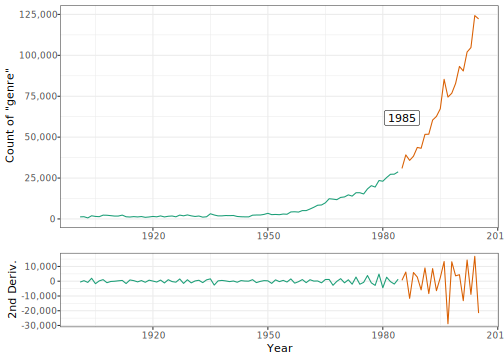
\includegraphics{ambrose_dissertation_files/figure-latex/ttsgnr-1} 

}

\caption{Historical frequency of term "genre" from Google Ngrams English corpus. Segments connote a change in acceleration (second derivative).}\label{fig:ttsgnr}
\end{figure}

Genre is a loanword from French. The origin of the French-Latin word
``genre'' and the English-German word ``kind'' both mean membership by
inheritance of innate class characteristics, archaically by presumptive
blood descent within a family, race, or nation. In common English it is
restricted to mean a broad category of art, especially literature and
music, and some but not all other cultural fields (e.g.~baseball is not
a genre of sports). As a term in scholarship, genre may be an observable
phenomenon, a conceptual component of a theory, or a conflation of the
two. In the social sciences genre is a specialty concept as in
sociology, while in the humanities it is ubiquitous especially in
cultural studies. Academics define and use the term differently between
and within disciplines.

\begin{figure}

{\centering \includegraphics{ambrose_dissertation_files/figure-latex/genre-goog-1} 

}

\caption{Wordcloud of third term in 3gram beginning with "genre of". Source: Google Ngrams}\label{fig:genre-goog}
\end{figure}

Figure \ref{fig:genre-goog} gives an indication of what things the term
genre has been used to describe. It illustrates the frequency of terms
appearing in the Google Books Ngram corpus as the third term in the
trigrams beginning with ``genre of'' or ``genres of''. The size of the
words is proportional to the total frequency of the trigram in the
English corpus, which spans centuries from 1590 to 2008 \citep{Google}.
The bias of the source--books--is clear in the outsized importance of
``literature'' and ``writing'' which are followed closely by ``music''.
The next ten largest nouns are poetry, discourse, fiction, art,
autobiography, painting, film, romance, folklore, and history. Ranked
within that series would be several adjectives as well: popular, science
(fiction), historical, and literary. Only on

To impose a sociological gloss on the term, these varied uses of genre
would make reviewing the literature on the topic difficult, were it not
for the discipline structure of the academy. The uses of the term genre
are themselves systematically organized by discipline, and a disciple
who is adequately trained will know the correct ways to use the term in
her local context. To use genre as a disciplinary convention means to
first identify your location in the disciplinary field, and then to
accept the limitations on scope by excluding those treatments of the
term that are extradisciplinary, that is, irrelevant. Disciplinary
structure reduces the true cultural complexity of the meaning of genre
to a restricted form, which in turn allows humble knowledge workers to
engage upon a set of shared assumptions. Such simplicity begets new
complexity as disciples spin out the consequences of their local use of
genre.

In the sociology of culture, genre is a form of classification enacted
by people in various social contexts. In the context of industrial
capitalism, genre is an economic principle helping to organize supply
and demand within markets for cultural products. There actors see genres
among the borders between economic, social, and cultural uses, as a
market category helping them acquire or produce content, as a card in
proximate games of prestige, or as something to taste, to consume and
enjoy directly. Less often genre is knowledge, a component of culture
separate from taste, that is a factor in the formation of ideas and
skills, whether these lead in turn to economic production or not.

Genre's meaning is context specific and variable across sociological
subfields, though it is amplified in empiricist fashion by economy and
society approaches that reduce genre to the act of classification
itself. I say empiricist because of the empirical ease with which the
classification or labeling actions are observed. Especially with
Internet distribution systems, it becomes trivial for corporations to
observe when a consumer labels her preferences while browsing a content
catalog; it is much harder to observe the ideas that consuming a
particular piece of content sparks in the mind.

In cultural studies genre is used much differently and much more in
accordance with its etymology. To the humanist, genre is an ontological
phenomenon, which is to say, genres are differentiated from each other
by combinations of discrete features of signs and signifieds. Humanists
are trained to establish these ontologies through methodological
readings of texts and through cultivation of theories of genre types.
These methods are at the same time empirical and interpretive, because
in consuming objective texts the researcher actually observes the ideas
that form in her own consciousness, and they may hope that others have a
resonant experience. Genres have more substance to them for humanists
than they do for sociologists. For sociologists of culture, genres are
how people use genre labels, while for humanists, genres are knowledge.

As we have said, the meaning of genre for a sociologist of culture is
economistic, at the same time a market category and a taste
configuration for consumers. The term differs for a sociologist of
knowledge, and perhaps for a cultural sociologist. It is ontology as it
is for the humanist, however it is not the ontology as represented to
the researcher in the consumption of texts. It is the hopelessly
unobservable distribution of ontologies appearing in a population of
consumers attending to similar texts. The sociologist of knowledge
accuses the sociologist of culture of reducing internalist concepts,
thought and experience, to externalist ones, taste and preference. The
sociologist of culture rejoins, show me proof, and on and on the
interlocutors spin around the axis defining the boundary between their
subfields.

But this description of subdisciplinary differences really is just an
example of a structural theory of genre that is within scope for the
sociologist of knowledge and beyond it for the sociologist of culture,
due to their epistemological differences. If genres are ontological,
then they deeply structure a person's experience of reality. Ontologies
form basic perceptual categories, and people with different ontologies
of an object experience different things even if oriented to the same
objective phenomenon. A ontological theory of genre would, for example,
attempt to explain differences in taste as differences in
phenomenological perception, whereas a taste theory of genre treats
consumption behavior as revealing preferences whose downstream
consequences are then explored.

Yet for all the differing treatments of genre mentioned above, do these
views of really contradict, or are they in fact complementary? Does
genre as distribution serve the economic sociologist's goals, or does a
lack of ontological substance lead her astray? Does genre as knowledge
remain hopelessly unverifiable, or are theoretical constructs necessary
to achieve a correct interpretation of facts? Is everyone at the club
listening to the same song hearing the same thing?

\hypertarget{disciplines}{%
\subsection{Disciplines}\label{disciplines}}

To return to disciplines, answering such questions would put the
researcher in an adisciplinary predicament, for it would mean eschewing
the scope restrictions cherished by disciples. The challenges of a
meta-disciplinary analysis are manifold and uncertain. One is as likely
to grow her audience as to lose it altogether. She risks the
dilettantism of a jack-of-all-trades. What's worse, she exposes herself
to a dizzying scale of content to consider. If disciplines are indeed
functional, then the meta-analysis that effaces disciplines risks being
dysfunctional. The upside, however, is appealing. If the universe of
meanings given to the term genre does contain complementary uses, a
meta-analysis will allow one to consider the consequences of the now
arbitrary segregation of a superior metaconcept across disciplinary
boundaries. Both sides of the divide could be strengthened by a cultural
exchange of their respective terms. The redundancy of parallel discovery
can be avoided.

Pathologies of disciplinarity can be diagnosed and treated. Disciplines
are social substructures embedded in a larger society and culture. If
disciplinarity is a kind of controlled ignorance exchanged for access to
secret knowledge. The wayward uses of a term like genre are always
lurking at the edges of the firelight defined by a particular
disciplinary camp. Discipline as rigor instructs disciples to resist
flirtations with the available complexity of the term. The essential
tension is very rarely between what is known and unknown; rather it is
more commonly between what is known ``here'' versus what we are
conditioned to be willfully ignorant of ``there''.

In a motivation of some of the arguments to follow, I take a
metadisciplinary approach, which is to cast as wide a net as possible on
the term genre. In so doing I hope to test the tacit cultural assumption
that discipline-based decisions of relevance are valid, that is, that
when we exclude arguments from other disciplines we remove distractions
and focus on what is important. The alternative possibility is that we
are wasting intellectual resources, because to exclude important work
about our topic, even if it is codified in foreign terms, is to risk
ignorance and redundancy. The topic is genre and how disciplinary
boundaries form such that people using the same word nonetheless cannot
communicate effectively. They draw on different paradigms, which is to
say the term is not really the same term. What I hope to do is uncover
the knowledge contexts surrounding the terms, and map these contexts in
a way that enumerates the various communities of discourse and theories
constituting the term.

\hypertarget{method}{%
\section{Method}\label{method}}

As I have said, the first consequence of eschewing disciplinary
limitations is to bloat the size of the ``literature'' on genre, since
no uses of the term would be excluded. An empirical approach to the
standard academic convention of a literature review will help reign in
the scale and complexity of the task. My aim, however, remains practical
rather than scientific. The methods need to be good enough to yield
results that offer something new above a traditional literature review
relying on library search and disciplinary wisdom about what is
important. This is not because a scientific approach is undesirable, it
is that it is not yet demanded of ``the literature''. Sociologists are
not expected to take a sociological orientation toward the history of
their fields. Rather the literature review serves the social purpose of
taking a position in a field of cultural production. It is a listing of
a roster of political support and rivalry, and an advertisement to
attract a desired audience.

To take an empirical approach to the literature review would be
subversive were it not the first function of disciplinary genres to
render atypical draws from the archive irrelevant. Disciplinary
subfields, genres, are credentialed by secret sets of references, and
most comers are held at the door. This in and of itself can be subersive
of even more arbitrary club rules, namely those of educational pedigree,
such that anyone willing to invest in a presentation of the genre
definition will be granted access to the venues, if not the invisible
colleges, of the subfield. To be admitted to the arena is no gaurantee
of achievement within it, but it is a start. Nevertheless, the scale of
the archive will always supply entropy enough to create a deterrent of
flotsam and jetsam around subfields composed of projects and persons who
either never cracked the code or who willfully eschewed it.

\hypertarget{distant-sampling}{%
\subsection{Distant sampling}\label{distant-sampling}}

The research strategy here attempts to parry the entropic tendency of
the archive by substituting human for machine limits. The time honored
methodological premise of a meta-analysis of genre is that the Gordian
knot of the global cultural complexity of the archive can be cut by
stratified sampling. I use a large digital archive of texts, JSTOR, to
represent the whole of the academic archive. Though clearly a toy
representing only a fraction of all networked scholarly produce, JSTOR
is large enough to easily surpass individual cognition and compel the
equivalent types of complexity reduction facing any researcher
approaching the real archive via their local university library portal.

I use a simple term search of the keyword ``genre'' to define half of a
sampling frame.\footnote{TODO, I did not, but should take a random draw
  of the same size to serve as a control.} I could then take a simple
random sample of texts, analyze how each uses the term genre, develop a
classification scheme, and enumerate the different uses of the term.
Unfortunately, a small sample in a statistical sense may be larger than
a poor researcher can handle. 1,000 texts is not large statistically,
but it is huge from a content analysis perspective. What's worse, 1,000
texts may still exclude, by random chance, small subcultures of the
term. Stratification resolves this issue by delineating those
subcultures so none would be left out.

Alas, the JSTOR digital archive lacks subject labels at the article
level, though it does include them for book chapters and for journals.
While not foolish, inheriting a journal label to the articles included
within it may be a coarse approximation if within-journal content
variation exceeds between-journal variation. We can use text analytic
classification methods to cluster articles directly and discover latent
groups of articles, and in so doing we can have an independent standard
to compare to the discipline labels given to journals. It is an open
question whether such methods align with what we have discussed above as
disciplinary and subdisciplinary groupings, for us whether regularities
in vocabulary correspond to regularities in the meaning of the term
genre. If they do not, then the study will only be a stop en route to a
true census of the uses of the term genre, and the contribution will be
to have interrogated the quality of the methods used, though this would
be a small consolation indeed!

The choice in computational text analysis (CTA) about how to represent
texts as data hinges on whether word order is preserved. The older and
more tested approach is to not preserve word order. The name given to
this ``bag of words'' format reminds one of its inelegance. A bag of
words is a frequency table for each document counting up the number of
times particular words are used, a representation that effectively
reduces a text to its vocabulary. It is the analyst's crude operational
decision to treat vocabularies as indicators of meaning, but social
scientists conventionally insist on cross validation via qualitative
analysis. While the ambitions of computational text analysis may start
with a replacement of, for instance, the standard literature review, the
conventional distrust, at least in sociology, of mathematical models of
text makes CTA more of a sampling method than an analytic method. The
study will culminate in a reading of texts, albeit one that is different
than traditional qualitative analysis because the CTA researcher
welcomes the introduction of interpretive bias from an understanding of
the mathematical model before, during, or after the texts are read. In
the game of ``choose your influence'', CTA is one choice while
disciplinary wisdom is another.

There are two types of classification methods in text analysis, direct
document clustering and topic modeling. Direct document clustering
treats the bag of words as a vector space and calculates distance or
similarity metrics between documents, which are then clustered. In a
topic model, the relationship between documents is mediated by an
unobserved but latently modeled representation of their content;
documents are similar because they are formed from the same topics.

Whichever approach one takes, and both may be used, recall that the goal
is to organize the texts into strata for the purpose of stratified
sampling. We said that we wish to typify and enumerate the different
uses of the term genre. By qualitative analysis, we could read every
text in a simple random sample and come up with a theory of the use of
genre in that text. The demerits of this approach are several
\citep[c.f.][5]{Nelson2017Computational}. It would take longer than we
want even for too small a sample. We are not humanists and have not been
trained in text analysis (this will hound us no matter what). Fatigue
will set in, and accuracy and consistency will suffer. We may limit our
set of theories to spare us the agony of complexity. It will be hard to
reproduce our results. There may be path dependency with a different
reading order producing different theories. On the upside, we would be
more educated for it.

Instead, we will stratify the sample, and it is in the configuration of
the strata that much of the work will be done. The strata impose upon
our interpretation of the texts the assumption of sameness.

\hypertarget{arms-length-reading}{%
\subsection{Arms-length reading}\label{arms-length-reading}}

The radical (and often maligned) distant reading approach taken by
digital humanists is being taken up with gusto by social scientists who
are less skeptical of quantitative methods. Following Nelson
\citeyearpar{Nelson2017Computational} I employ a quantitative analysis
of texts not to replace human reading with machine reading but to
support reproducibility in traditional qualitative content analysis.
While CTA makes it possible to dispense with reading altogether,
knowledge, understanding, and the cultural logics of
arguments--especially their ontologies--are still only obtainable by
reading primary texts, closely or not. The most radical interpretive CTA
method would involve deep neural net supervised machine learning, which
may be able to predict how a particular human reader would classify a
text without their needing to read it, though this has never been
demonstrated. What I gain from CTA is guidance in answering the question
of what to read, and perhaps in what order to do so.

As we know, the question of what to read is answered institutionally for
scholars already by way of canon, curriculum, word of mouth, and digital
reference term search services. These are their own forms of distant
reading, because they each make obsolete the archaic image, true of
figures like Weber, of a scholar buried in library stacks reading
everything they come across (and so it has been said of Weber,
forgetting nothing).\footnote{What a scandal it would be if Weber's
  lionizers discovered that he had only read text indices! Surely they
  would bury such a fact. But the point would remain that even if a
  scholar were able to consumer an entire corpus, the sheer scale of
  contemporary publication is now beyond even a genius's capacity.}
These contemporary shortcuts are historically arbitrary, but what is
important is first that they serve the function of reducing the
overwhelming cognitive complexity of published scholarship, and second
structure that reduction in the same way for all scholars. An arbitrary
reduction needs to be consistent to act as an infrastructure for
subdisciplinary scholarship, otherwise scholars would find themselves
located in different literatures.

If distant reading is a criticism of close reading then it has a big
hill to climb especially among humanists who are trained to deal
methodically with texts very carefully. In the social sciences a type of
customary distant reading is that of ritual citations, those that have
developed a meaning that may be oblique to their content or at odds with
the intentions of the the original authors. A ritual citation is simply
one that is cited but not read, but also one that is so often used that
its socially acceptable usages are known from other secondary accounts.

What are the social patterns of the traditional literature review are
topics for the sociology of knowledge and science and for the
information sciences. This is not the task of the current study. What we
take from the traditional approach is the consequences of excluding
large segments of intellectual history. What CTA makes possible for the
first time is a nonarbitrary, inclusive analysis of \emph{all} content
in a digitized corpus. It will not necessarily be a good analysis, but
what it will lack in quality it will make up for in coverage. A CTA
approach to the literature review will at least make clear what lacuna
would be left by the traditional approach. They also reduce the
potential idiosyncrasy of a particular author's literature review
because, unlike a personal reading, a CTA model can be communicated
precisely.

Of course the cognitive limitation of how much any scholar can actually
read and understand remains. There will be an exclusion mechanism no
matter what, therefore a chief assumption of a CTA literature review is
that corpus segmentation is both possible and that some reduced form of
reading, some sampling procedure, can be said to be representative of
the unread portion in each segment. If on the contrary no two snowflakes
are alike, then the enterprise of knowing more than we have before is
fraught, and CTA becomes yet another arbitrary reducer.

What's worse, or perhaps better, is that there is reason to believe that
idiosyncrasy itself is an historically variable feature of disciplines.
If institutional isomorphism has proceeded to some high level in
contemporary disciplines, then the assumption that reading the
bellwether texts is as good as reading the entire herd may hold. If this
is true, however, it raises as many questions about the process of
institutionalization in cultural production than it answers about the
potential to learn truer versions of intellectual history.

\hypertarget{topic-models}{%
\subsection{Topic Models}\label{topic-models}}

We have referred generically to computational text analysis, and now we
can discuss the topic model as our technique of choice. There are many
ways of estimating a topic model (e.g.~the famous Latent Dirichlet
Allocation or LDA estimator) but the model itself is simple. It is a
latent variable model that decomposes a document-by-term matrix--in
which every document is represented as a frequency distribution over
every term appearing in the corpus--into two unobserved matrices:

\begin{itemize}
\tightlist
\item
  a topic-by-term matrix, and
\item
  a document-by-topic matrix.
\end{itemize}

Topics are directly represented by they topic-by-term matrix. A topic is
a probability distribution over a vocabulary. To draw on a topic means
to choose vocabulary as a random draw from this distribution, where
words with higher probabilities will be chosen more often. In the case
of genres we might imagine a topic about film and a topic about music.
Some words may be important (highly probable), to both topics, such as
the word ``genre'', while others would be distinct, such as the words
``movie'' (probable for film but improbable for music) and ``band''
(vice versa).

Given topics as term distributions, a document can be represented not as
a distribution over terms, but as a distribution over topics. The topic
mediates the relationship between documents and terms. In order to
generate diction for a document, all that need be understood is the
ratio of topics out of which it is composed. This is sometimes explained
as a generative mechanism; to ask what word will be chosen next in
composing a document, one first samples from the document's own topic
distribution to decide which topic the word will be drawn from, and
given that topic, one then samples from the topic's word distribution to
decide which word will be included in the document. A document's topic
probabilities also create the expectation of how many words are
attributed to eac topic. A document with topic probabilities .7 from
music and .3 from film would be 70 percent about music and 30 percent
about film, making for a parsimonious albeit reductive description of
document content.

It is important not to overinterpret a topic model. Topic models are
sometimes called ``generative'' as if they explained how documents are
written. Such a generative metaphor reveals the absurdity of a topic
model as a representation of writing. Not to mention the fact that
punctuation tends not to be represented (though it could be), the terms
chosen would be in a random order incapable of making meaningful
sentences. Hence it is best to avoid the generative metaphor as an
explanation of texts. If topic models touch on the generation of real,
meaningful documents, it is only a very limited sense. What the topic
model really represents is how vocabularies are organized to condition
an author's diction. A vocabulary can be thought of as an infrastructure
of meaning more trivial than grammar or syntax. A topic is a simple list
of words that is known or knowable across all authors in a field. Topics
do not tell stories; authors tell stories in part by making diction
choices that are conditioned by topics.

From a sense or meaning making perspective topics are trivial; this is
because so little is known about what an author says by knowing the
topic or even the term distribution of a document. What topics are
useful for, however, is the type of segmentation or cartography of a
corpus. Topics are really a global feature, perhaps a cultural feature,
of a corpus of texts that is itself meaningfully selected. If indeed a
field of texts is oriented to common if not always overlapping
vocabularies, then topics can represent this well.

A topic model could be posited based on the domain knowledge of an
expert, and this would be a form of estimation. The practical value of
statistical topic modeling is that the unobserved topics can be induced,
with a raft of assumptions, directly from the observed document-by-term
matrix to arrive at a model with the features just described. An
estimated topic model will contain several other parameters filling in
assumptions necessary to make it possible to identify the unobservable
topic probabilities in each of the two matrices of the model. For
instance, the parameter commonly called alpha makes an assumption about
how many topics tend to comprise each document. s

\citep{DiMaggio2013Exploiting}

\hypertarget{data}{%
\section{Data}\label{data}}

We will use the JSTOR Data for Research service to download a
bag-of-words text corpus for topic modeling. I take the following steps
to develop a corpus:

\begin{enumerate}
\def\labelenumi{\arabic{enumi}.}
\tightlist
\item
  Search dfr.jstor.org using the query
  \texttt{(ta:genr*\ OR\ ab:genr*)\ AND\ la:eng} and requesting 1grams.
\item
  To cull documents for which genre is not an important term, exclude
  documents containing fewer than five variants of the term genre
  (1grams matching the regular expression \texttt{\^{}genr}: genre,
  genred, and genres).
\item
  Remove ngrams appearing fewer than three times, which often includes
  optical character recognition errors.
\item
  Remove ngrams shorter than three characters and longer than 25
  characters, again often OCR errors but also stopwords that will be
  removed anyway.\footnote{The Freudian ``id'' is an unfortunate
    casualty of this step, as well as some footnotes, endnotes, and
    captions containing small text where word boundaries were not
    detected during OCR and a series of words was concatenated.}
\item
  Remove ngrams longer than three characters that are all the same
  letter, often OCR errors but sometimes real, as in Roman numerals.
\item
  Compile baseline word counts for each document assuming that at this
  step the documents contain only valid terms, and no OCR errors.
\item
  Remove SMART stopwords.
\item
  Remove numbers.
\item
  Remove punctuation, except intraword hyphens.
\item
  Lemmatize or stem English words.
\item
  Remove lemma with fewer than three characters.
\item
  Aggregate 1grams defined by a single lemma and, for ease of
  interpretation, name the sum after the most common 1gram.
\item
  Remove terms appearing in fewer than 20 documents.
\item
  Remove documents that, after the above filters, have a word count of
  fewer than 500 words.
\end{enumerate}

The initial query returned 7,695 articles from 1,205 different journals,
as well as 6,485 book chapters from 4,427 books. After the above
processing steps, the sample was reduced to 3,545 articles and 2,799
chapters, or 6,344 total texts.

It is fair to ask what is lost during the pre-processing of texts. Many
are included in error due to JSTOR's internal translation of abstracts;
where ``genre'' is the French translation of the English ``kind'' the
text will be included even if the term genre does not actually appear in
the English title or abstract. While I do not carefully look at the
content of the excluded documents, assuming they were not texts that
made important use of the term genre, I do retain some information about
what components of a text were lost of those documents that were not
cut. This is a measure called idiosyncrasy, or the proportion of terms
in a document eliminated during pre-processing. I call it idiosyncracy
because the pre-processing condition was that terms would be eliminated
if they did not appear in at least 20 other texts. Texts that lost a
large volume of words to this filter are drawing on a vocabulary that
almost no other texts use. It would not be surprising if these were
ethnographic or content analytic studies of non English materials.

Figure \ref{fig:idi-hist} shows the right-skewed distribution of
idiosyncracy. The median text lost about one tenth (10.16 percent) of
its words, while 90 percent of texts are within two tenths, and outliers
begin at about three tenths as can be seen in the boxplot. The 150 (2.36
percent of) texts above three tenths vary across a range as wide as the
rest of the distribution. The most idiosyncratic text, at 60.4 percent
of its vocabulary lost, is Pelli's ``The Revival of the Literary Genre
of Religious Disputation in Hebrew Haskalah: Isaac Satanow's
\emph{Divrei Rivot}''.\footnote{www.jstor.org/stable/10.2307/27909026}
The article, from the journal \emph{Hebrew Studies}, is a single page
introduction in English to a 12 page essay reprinted in the original
Hebrew. By page count alone we would expect the idiosycrasy to be 12/13
or 92.3 percent, which also illustrates how terms that are not in the
Roman alphabet may be discarded as OCR errors even prior to the
idiosyncracy measurement.

\begin{figure}

{\centering 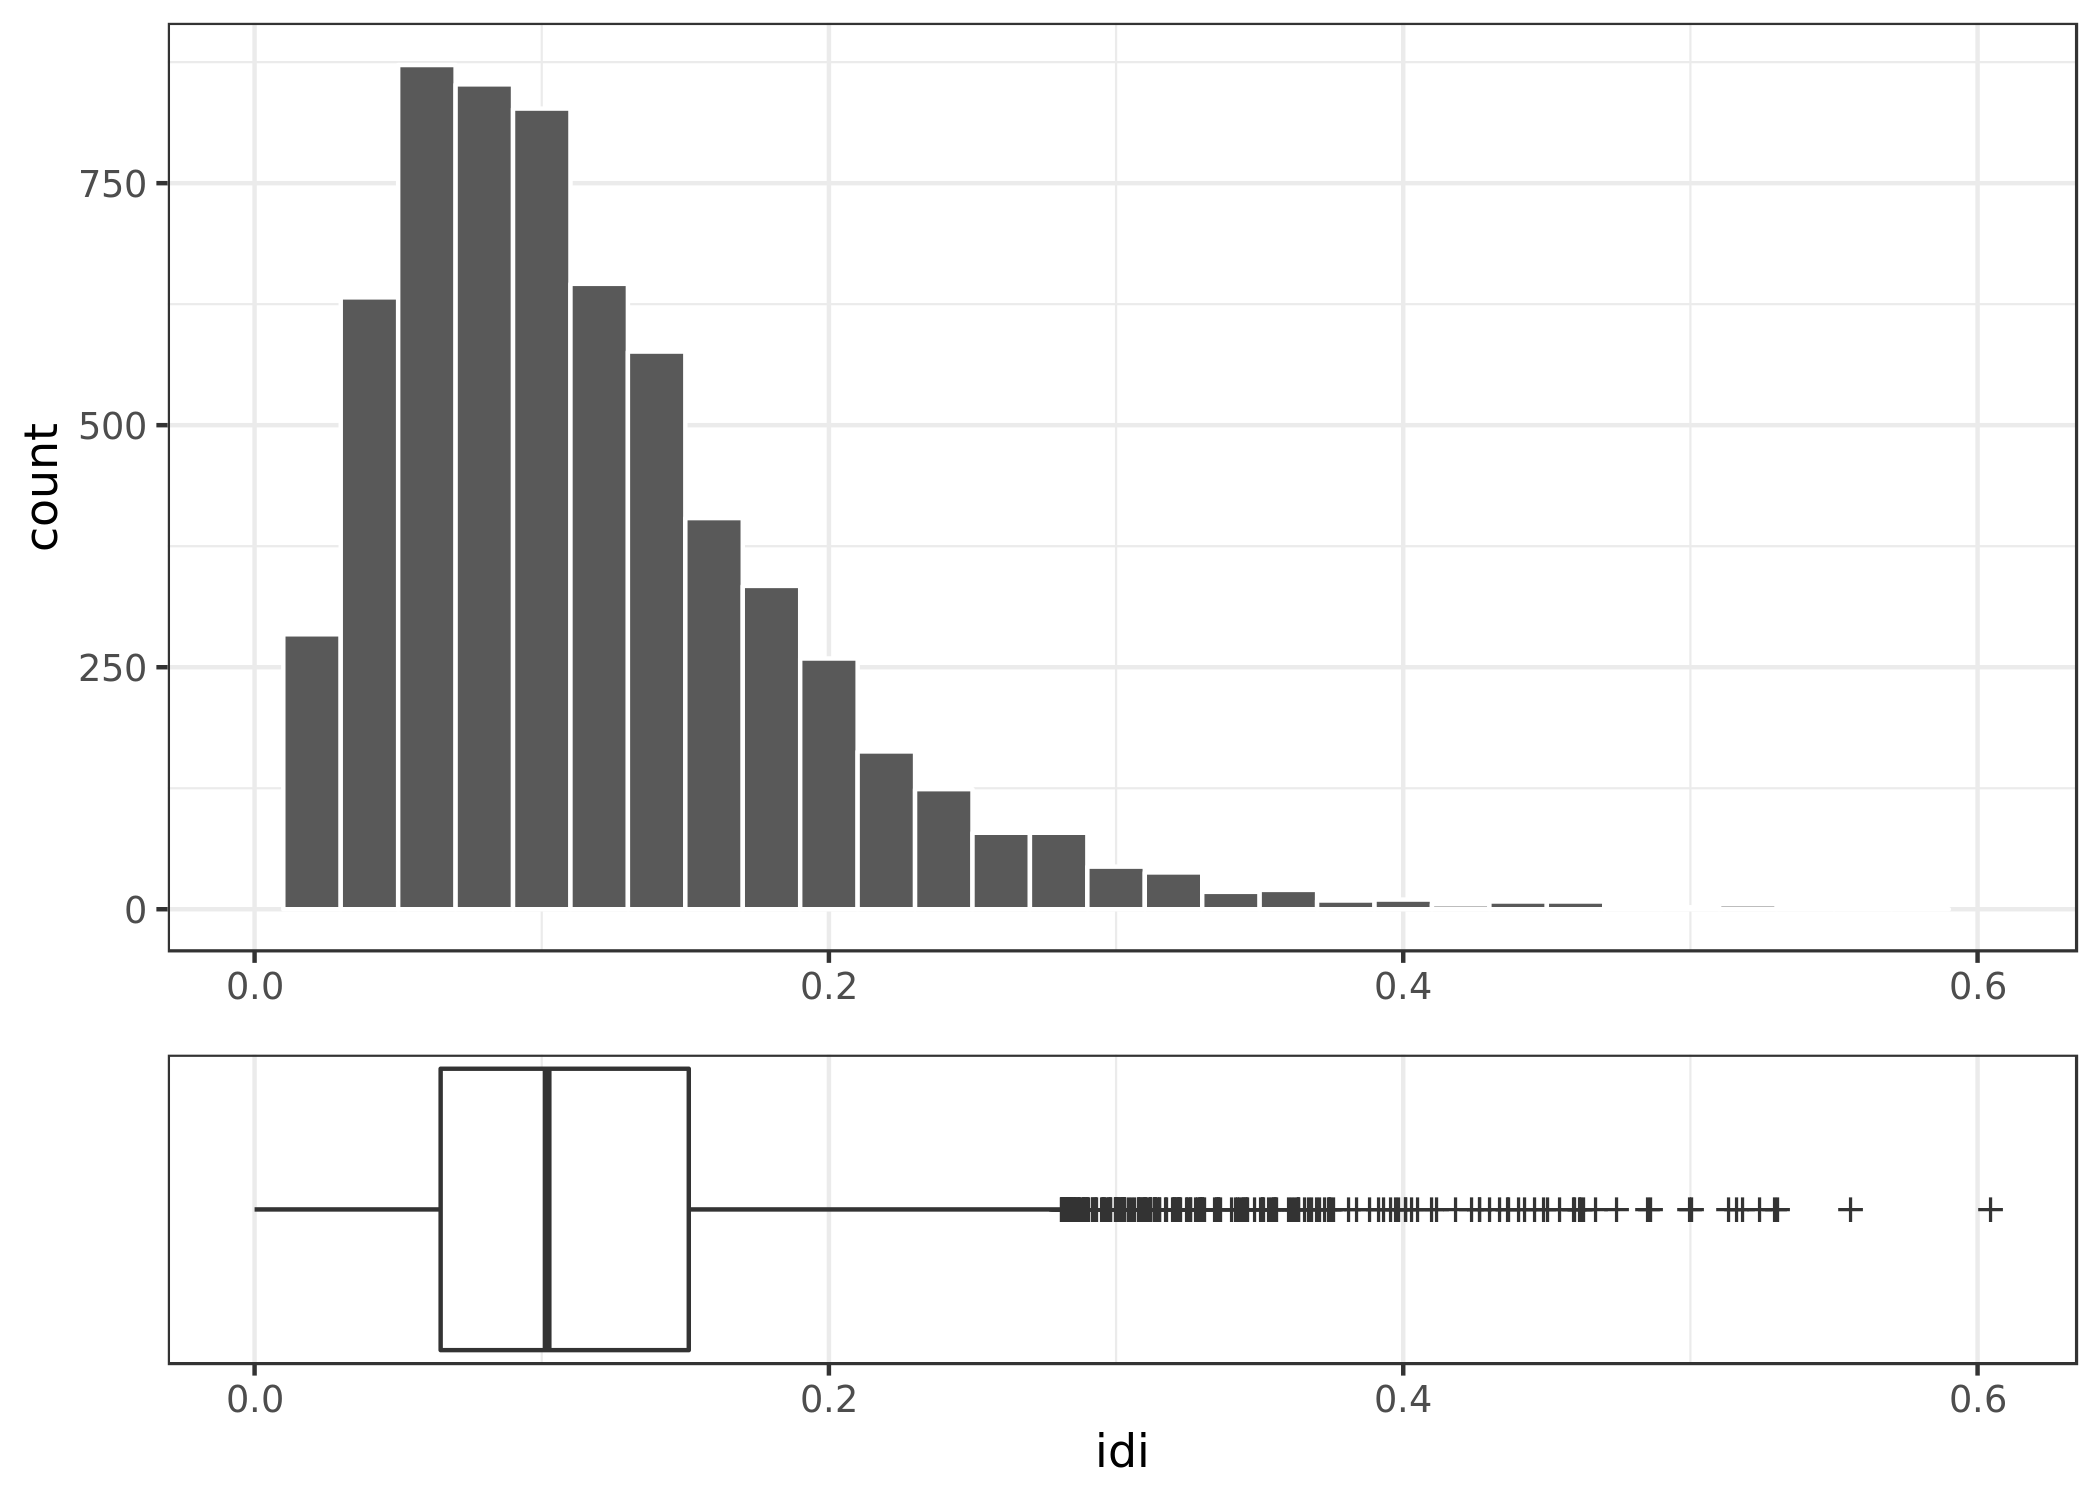
\includegraphics{ambrose_dissertation_files/figure-latex/idi-hist-1} 

}

\caption{Distribution of idiosyncracy, the proportion of document vocabularly dropped during pre-processing. Pluses indicate outliers.}\label{fig:idi-hist}
\end{figure}

Figure \ref{fig:gp-hist} shows the logarithm of the count of the term
genre as a proportion of the total term count of a text. This
distribution is much more highly skewed but contains fewer outliers. In
the median text a genre variant accounted for about 6 in 1,000 terms,
while at the 90 percentile the rate is 27 in 1,000. 46 texts (0.73
percent) are outliers where one in ten or more words is a genre variant.
The text with the largest genre proportion, at 35.7 percent of its
words, is Welsh's ``Editorial: The Genre Revival''\footnote{www.jstor.org/stable/10.2307/43795866}
is a single page introduction in a special issue of
\emph{Literature/Film Quarterly} on genres.

\begin{figure}

{\centering 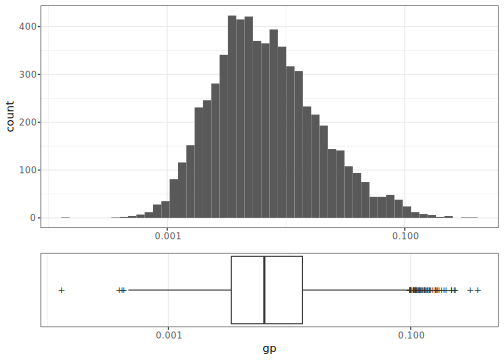
\includegraphics{ambrose_dissertation_files/figure-latex/gp-hist-1} 

}

\caption{Distribution of $log_{10}$ of the count of the term "genre" as a proportion of all terms in a text. Pluses indicate outliers.}\label{fig:gp-hist}
\end{figure}

\hypertarget{sankey}{%
\section{sankey}\label{sankey}}

Topic models require the analyst to choose the number of topics \(K\).
The approach we take to guiding this decision is not to expect one
correct specification of K but rather to see it as a changing
resolution. A K=2 model usefully bifurcates the sample and is not wrong
because it is too restrictive. As K increases we expect the samples to
continue to divide as new parameter spaces become available to partition
the sample. While this is not strictly a hierarchical design, since each
K model is fit independently, we should expect to see aspects of
hierarchical topics as well as some degree of stability in the
relationships among topics.

Categorical Expectation Maximization is known to

\hypertarget{top-x-doc}{%
\section{top x doc}\label{top-x-doc}}

\begin{figure}

{\centering \includegraphics{ambrose_dissertation_files/figure-latex/unnamed-chunk-9-1} 

}

\caption{Sankey diagram of document overlap between topic models of increasing values of K.}\label{fig:unnamed-chunk-9}
\end{figure}

\hypertarget{gen}{%
\chapter{Social Science Genres Today}\label{gen}}

\hypertarget{abstract-1}{%
\subsubsection*{Abstract}\label{abstract-1}}


Social science is arranged into disciplines in a manner
strikingly similar to the genre systems of commercial fields of cultural
production (FCP) like music, yet evolving at a slower pace. Genres
appear static and given in the form of the labeling schemes of
archivists and librarians. Such schemes aim to describe academic genres
objectively, yet in so doing referencers and indexers reify them
historically. Such genre classifications are at times useful,
frustrating, or didactic for the academic ``disciples'' or knowledge
workers of higher education. This study maps the cognitive system of
genre classifications in one particular labeling scheme, that of the
JSTOR historical archive, as applied to one aspect of academic FCPs,
journals. The patterns of interdisciplinary cross labeling, of allowing
journals to bear multiple labels, reveal how global axes among science,
social science, and humanities condition the local relationships of
disciplines like sociology and anthroplogy.

\hypertarget{keywords-1}{%
\subsubsection*{Keywords}\label{keywords-1}}


genre, social science, knowledge mapping, labeling,
cognition

\hypertarget{introduction}{%
\section{Introduction}\label{introduction}}

\begin{quote}
The science that everybody is\ldots called upon to possess hardly
deserves that name. It is not science; or at the very most it is the
most common and general part of it. It is indeed limited to a few
indispensable elements of knowledge which are only required of everyone
because they are within everyone's grasp. Science proper soars
infinitely beyond this vulgar level. It includes not only what one would
blush at not knowing, but all that it is possible to know. It presumes
among those who are its adepts not only those average faculties
possessed by all men, but special aptitudes. In consequence, since it is
accessible only to an elite, it is not obligatory. Although something
fine and useful, it is not so utterly indispensable that society
categorically requires it. There is advantage in being equipped with it,
but nothing immoral about not acquiring it. It is a field of activity
open to everyone on their own initiative, but one which no one is
compelled to enter. One is no more required to be a scientist than an
artist. \citep[43]{Durkheim1893division}
\end{quote}

Genre is a both a phenomenon and an analytical approach, indeed, several
analytical approaches. I critique a contemporary use of multimodal
network analysis to study genre as measured in cultural object network
data. I argue that standard rational choice approaches in the sociology
of culture, the theory of consumer preferences or tastes, does not pass
a prima facie test of validity as an accurate representation of the
global properties of so-called cultural networks. The same data that are
used to demonstrate taste theory better support an alternative knowledge
based approach to culture.

\hypertarget{taste}{%
\subsection{Taste}\label{taste}}

Lizardo operationalizes genre preference data in network terms by
``inducing a network of persons connected to the cultural genres they
choose'' \citeyearpar[53]{Lizardo2018mutual}. This allows him to analyze
individual preferences within a global context represented in bimodal
network patterns. Multimodal networks, of which a bimodal network is the
simplest type, are an analytical convention wherein at least two classes
of items bear relations and in which a rule is imposed that such items
may only be related to items of a different class. Insofar as the
researcher cares about intraclass relationships she must understand them
as mediated by one of the alternative classes.

This multimodal metric convention aligns with cultural capital theories
of culture which treat the consumption of cultural objects as
transactions out of knowledge relationships and into status ones. In a
knowledge relationship cultural logics obtain, usually a principle of
rightness like truth, beauty, or morality. Social relationships, on the
other hand, are governed by different rules, e.g.~those of commitments
like love and enmity or loyalty and rivalry. The meaning of a cultural
object is given by the interactions established around it, which are
themselves conditioned by role expectations
\citep[445]{DiMaggio1987Classification}. Cultural capital then is the
type of relationship process where an actor tries to exchange knowledge
for status as the basis for a relationship or at least to motivate a
particular role interaction.

This treatment of cultural capital differs from more strictly
Bourdieusian approaches. Serino et al \citeyearpar{Serino2017Bridging}
do it differently.

The simplest multimodal network has two classes (see
\citep{Shi2015Weaving} for examples of many more).

culture as a disembodied abstraction \citep{Lizardo2018mutual}

\begin{quote}
\begin{quote}
Genre classifications socialize the infrastructure costs of artistic
production. \citep[445]{DiMaggio1987Classification}
\end{quote}
\end{quote}

\hypertarget{structuralist}{%
\subsection{Structuralist}\label{structuralist}}

Genres are a feature of two kinds of cultural surplus. First, genres are
not necessary if knowledge is limited to a small number of lessons,
stories, ideas, or skills. Such a cultural corpus is naturally held as
``the'' obligatory culture, and because knowers do not experience
options they do not face the problem that genres solve. When such a
unary culture expands beyond the mental or technological limits of
memory, or when it is faced with alien knowledge sources, a proto genre
is functionally necessary that allows for a binary classification
between sense and nonsense.

Such a proto genre allows two things. Alien material becomes obvious,
perhaps dangerous, but not confusing as it can be safely cordoned off
from what is real knowledge. Second and perhaps more interestingly, a
proto genre precipitates cultural expansion by allowing some stories
(ideas, skills, products) to be told differently. Such novelty maintains
interest without exciting alienation. In those acts of deciding what
makes sense (inclusion) and what is nonsense (exclusion) the rules of
the genre begin to form.

When genres become multiple they cease to be about sense and nonsense
and begin to be about relevance and irrelevance. They allow local action
with a globalized culture by reducing local cultural complexity to a
manageable level, and what is more important, they make normative and
binding the particular pattern of exclusion. The genre classification of
particular cultural objects must be done correctly or they will invite
more or less predictable social backlash. In this way ``personal genre''
must be understood to be an oxymoron; a person may have tastes, her own
rules of repulsion and attraction, but to the extent that these tastes
abrogate genre conventions a person has difficult decisions to make
about how she will field the forms of social regulations, and perhaps
rewards, that she will incur in expressing those tastes.

This is not to say that socialized tastes, tastes that conform to genre
convention, do not incure regulation and reward. Indeed we will see that
one function of multigenre systems is to allow cultural industries to
minimize exclusion and maximize conversions. In this sense the
developmental model with which we began has a circular logic of scale;
as genre systems grow and differentiate in the vain attempt to index the
wild cultural content they hope to classify, industrial action lights
upon this natural tendency and works to domesticate it. In working to
exclude nothing, purveyors of culture demonstrate themselves to be
tastelessly willing to hock something to anyone.

This simple structuralism is a functional understanding of genres, which
though not a sensible analytical approach in contemporary sociology,
forms the spine of the argument to follow. The effect of genres that we
wish to focus on is their exclusion potential.

\hypertarget{culture}{%
\section{Culture}\label{culture}}

Bodies of knowledge and practice, cultures, exist because of yet apart
from particular people. While some cultures are ubiquitous and
inculcated in all members of the societies in which they are
substantiated, others are esoteric and marked by significant barriers to
learning them. Such esoteric cultures are as inaccessible as they are
unnecessary. A child who does not learn what to eat and how to eat it in
her local culture will have great difficulty doing anything else in her
society. Food culture is of the ubiquitous type and is not difficult to
learn. On the other hand, a child who does not master scripture will be
ashamed at temple, but shame is bearable in a way that hunger is not.
Scripture is of the esoteric type; knowledge of it enables special
abilities and grants access to restricted aspects of a society, but
ignorance of it does not threaten one's lay livelihood. Even in
religiously totalitarian societies, what religous knowledge is necessary
will be ubiquitous. What religious knowledge is esoteric can be safely
left to the clergy. It is not too narrowly circular to say that the
knowledge that informs daily life is the easiest to aqcuire, and that
the mere act of living also reproduces that knowledge within contexts
that are themselves ubiquitous. Whether relationships of ubiquity are
familial, economic, or state relations varies by society, but no society
lacks ubiquitous culture and the means of reproducing it.

Esoteric cultures, then, are removed from ubiquitous ones though they
depend on them. They require specialized social relationships for their
reproduction in populations. These special relationships may be called
fields of cultural production (FCP). FCPs are both reproductive of
extant knowledge and productive of novel knowledge relevant usually only
to the field itself. To the extent that esoteric cultures are
complicated or otherwise have high entropy, the failure to reproduce
their cultural content is always an existential threat. While it is a
gaurantee that cultural content is constantly actually lost to
reproduction failures, cultures that nonetheless persist historically
must always have a socially structured FCP that, in inculcating new
members and reinforcing the knowledge of extant members, resists the
entropic decay that would otherwise lead to extinction.

The scope of a culture has a knowledge and a social dimension. Units of
knowledge are both discrete and combinatoric. Discretely, the size of a
culture can be measured by a count of co-occuring ideas and skills. The
utility of knowledge, for instance as instantiated in an FCP, often
depends on the combination and interaction of such discrete elements.
The mass of knowledge in a culture is related to the count of units and
to the ease with which those units can be learned, thought, or deployed
in meaningful activity. Some cultures are easier than others, and it is
the effort-adjusted size that is the real mass of the ideational content
of a culture.

Not all sociologically relevant information is cultural. In the triadic
relationship among culture, social structure, and personality,
psychological concepts like schemata that are sometimes treated as
constitutive of social structure do not belong in the category of
culture. Schemata allow personalities to organize their responses to a
world that includes many things beyond culture. In order for cultures
and social structures to function stably in time, they depend on the
successful operation of schema, but they do not necessarily provision
these schema. An only partial exception is the limiting and very
specialized cases of pedagogical institutions. A culture can only exist
if people can reproduce it, but the people must solve the psychological
problems of cognition on their own. Whereas culture is fungible in its
different mediated forms, there is no reason to believe that a ``single
schema'' occurs across a population of people. There are no
one-size-fits-all solutions to human motivation, and schema will to a
large extent be idiosyncratic, adapted as they must be to the particular
circumstances in which people as träger find themselves.

What cultures can do to hedge their bets against the instability of
personalities is to introduce kinds of knowledge adapted to cognitive
problems. Schutz identifies systems of relevance from the side of
personalities, and here we understand the same from the side of
cultures.

People know culture and it does not appear apart from them. Put
differently, culture is information and people are the media that
concretely manifest it. The size of a culture is the count of the unique
ideas and idea combinations appearing in a deduplicated media catalog,
excluding possible but unrealized combinations. The potential of a
culture is the size of the realized and unrealized combinations, where
the number of elements in a set is limited by a given historical
cognitive and technological memory capacity. The potential of a real
culture is always greater than its size, as combination novelty always
easily exceeds the available media.

The social mass of the culture is the enumeration of the media in which
cultural content actually appears historically. The cultural mass is
copied piecemeal among a population of knowers. The mass may be enlarged
by information technology by making it easier to access and transmit
culture, but the artifacts and technology themselves do not count in the
mass of the culture. Real, historical human nervous systems, including
language expression,

Dead cultures cannot live again because the dead part, the social part,
is highly ephemeral. Even if a culture leaves material and symbolic
artifacts, the ``dead'' parts are precisely those human relationships
that would socialize new members in particular ways that cannot be
deduced by people who never belonged to begin with, namely the
archeologists of the future. Such archeologists belong to the FCP of
their own time, and approach the historical artifacts of a dead culture
as any other FCP approaches regular patterns in the world, as subject to
their own particular cultural logics.

Reproduction does not necessarily imply long term consistency of
cultural content, indeed a high level of knowledge loss may be a sign of
historical stability in an esoteric culture if it results from a highly
productive FCP. An oversupply of cultural content increases the chances
that some, any culture can be conveyed into the future in a chain of
descent.

Esoteric knowledge is essentially cryptic, ubiquituous knowledge
essentially evident. Crypticism means that layity cannot acquire
knowledge on their own, that is, without socially structured access to
an FCP. Esotericism is the social consequence of crypticism. Cultures
vary by knowledge features, as knowledge is a social axis of power along
which status hierarchy necessarily develops. Knowledge asymmetry
structures social relationships, usually leading to status inequality.

High entropy cultures must socialize new and maintain existing members
like any culture, but their complications also tend to be generative of
novelty.

The ubiquitous cultures will be learned because there is nothing in a
society to do without knowing them, while esoteric ones are gauranteed
to be forgotten by most, swapped easily for the always ready ubiquitous
alternatives. Ubiquitous cultures have high ambient findability
\citep{Morville2009Ambient}, they can be transparently acquired for
instance through mimicry \citep{DiMaggio1983Iron}.

FCPs are social structures that can be thought of as the articulation
points between people and a special type of culture that we associate
with higher education.

To be sure, if esoteric cultures are marked by asymmetries of knowledge
between laity and clergy, to continue with the religious example, we
must admit that such asymetries exist in ubiquitous culture as well, as
in the supposed ignorance of a child against the learning of an adult.
The ignorance of children combined with their megalomania is a useful
example of how social structures operate. Social structures are always
culturally conservative; a child's ignorance is a generative force, as
they may attempt to solve problems in novel ways, and their efforts will
frequently be corrected by the experts. Whether the correction takes
marks the chagrin of the parent. Children quickly become specialists in
their own FCPs, but this is never because they aren't also aware of the
ubiquity. They may know it, it may bore them, and they efface it for
fun. But they know what is ubiquitous; their proximity to ignorance of
it may animate their creative abrogation of culture. The essentially
conservative function of pedagogy will stamp out that creative flame in
time. Indeed children are a great source of entropy for ubiquitous
culture, hence the large investment in education generally.

This evolutionary argument can be more simply stated as, complicated
cultures cannot exist for very long without stewardship.

\hypertarget{genre-profession-and-cultural-morphodynamics}{%
\section{Genre, Profession, and Cultural
Morphodynamics}\label{genre-profession-and-cultural-morphodynamics}}

Genre in sociology has been treated from literary, economic, and
historical vantages.

Economic sociology has treated genre as an integrating feature of
markets, expressed simultaneously by both supply side and demand side
actors \citep[441]{DiMaggio1987Classification}. DiMaggio posits an
oversocialized conception of artistic classification systems that sets
genre as a matching between consumers on one hand and production,
including producers and distributors, on the other. Consumption of art
is essentially transacted for social goods, that is, is a form of
cultural capital. Because cultural products are objects of ritual
satisfaction among consumers, social relations are limited to
intra-economic categories. This is the same as saying that social
boundaries mark cultural boundaries. The meaning of cultural products to
producers is very different than to consumers, there is no cultural
logic that transcends social boundaries, that is, there is no ``cultural
totality'' even at restricted scales.

Whether this is an accurate depcitions of the arts, it is not adequate
for direct adaption to the analysis of scholarly disciplines. The
missing variable is the pedagogical nature of social relationships. In
pedagogical relations assymetries of cultural understanding are built in
to the role structure of social relationships.

The professional relates to a client. The administrator relates to a
subject. The purveyor relates to a customer.

This may be an accurate

DiMaggio discusses three organizational forms--commercial, professional,
and administrative--as explaining gen

\hypertarget{generic-vs-typical}{%
\subsection{Generic vs Typical}\label{generic-vs-typical}}

Following Schutz all cognition is process that begins by matching
knowledge to experience via an intial process of typification. Empirical
objects are categorized according to types, and our knowledge is also
indexed according to those types. We know what to do once we have typed
an object and matched it to type organized knowledge.

Genres

In non market societies, FCPs are financed by state patronage. Here
esoteric cultures that have no need of a laity will be invisible to most
of the members of the society, and their knowledge will be naturally
excludable. Market societies organize

\citet{Schutz1970Reflections}

Beer \citeyearpar{Beer2013Genre} posits genre as a form of Foucaultian
classification where a formal ``grid'' of knowledge structures
observations while inviting subversive criticism. Missing in the use of
Foucault is a sense of historical transition between types of knowledge.
Scientific knowledge passed through stages limited by new concepts of
order. The grid or classification logic was replaced by causal logic in
a process spanning generations. \citep[150]{Foucault2002order} Reading
Foucault as a developmental theory means that a classification logic
provides the knowledge necessary to envision a causal logic. In this
sense, a reified and possibly stitled genre classification system is
generative of a more nuanced causal logic in that it provides an anchor
and set of easily workable tacit arguments; sociology is different from
anthroplogy because of a deployed catalogical schema. Beer however puts
formal and informal genre systems into an ahistorical relation; formal
genres are not generative of causal explanations of genre, but rather
they are power structures against which interested actors struggle to
either support or efface.

Foucaultian genre requires a method of description, and the components
of the method describe or order observations of the thing. Genres do not
work this way except in a post-hoc way, as the recent controversy over
the single Country Road illustrates. Genres in this sense actually work
as a pre-classification Classical system, as pure language in which
knowledge is knitted together by merely tracking down uses of the term.
Genres amount to anyone's use of the genres as terms. Genre criticsm
operates in this mode; genres are leverged to inflrate deflate the
reputation of particular social alters. Far from describing the
characteristics of the music, genre as a term encompasses how the genres
are used, such as in their influence on scene formations and fashion.
These are primitive forms of knowledge if Foucault's account of science
is taken developmentally.

Marxian structural development classically contends that stages of
history cannot be skipped. Some theorists partially relax this model
with a version of structural memory wherein a society that has undergone
a transition into a particular stage of development, the resources
genreating the relationsihps of the previous stages are already
available. This is why development is slow first, but when the process
has been played it may be replayed at much greater speed, and it may be
played out of order. What is normally mapped to a process of time may in
an advanced stage be mapped to different dimensions. The one we will be
concered with is a status dimension. The classical form of knowledge,
wherein it is stiched together piecemeal by focus on the language, the
use of the term, leaving little coherence to the threads so collected,
is simple and available always. The more structure classificaiton
according to a rule-based grid is more advanced. Rather than being
available only in time, after it's invention, it may be aviaalbe as an
asymmetry of training or socializaiton. Grid-knowledge may be utilized
among the clerics and not available to the laity. At the core of the
clerics, the elite of the esoterics, the most complicated stage of
causal reasoning, is available to even fewer people. Boulding, in his
own genre scheme, called the same the distinction between frameworks and
clockworks \citep[202]{Boulding1956General}.

What this view allows us to ask is, for Beer's emphasis on the critical
use of genre categories, does it matter that the laity flirt with
classical kinds of knowledge. Does it, as Beer suggests, work to reform
the genre categories? Or on the other hand, to the institutions of
formal categorization easily ignore such debates, or do they rather have
aggreagtion systems of their own to handle ``deomcratic'' or market
research processes like genre term searches?

\hypertarget{kd-dq1}{%
\section{JSTOR Journals}\label{kd-dq1}}

Genre classifications are totalizing, as any factor or product in a
field of production can be labeled and sorted according to a categorical
logic.

We rely on the JSTOR digital archive which gives access to optical scans
of historical journals. JSTOR provides a title list of their journal
coverage \citep{JSTOR2018Title}. The coverage of journals in the archive
is very complete for those journals chosen for the database. As of this
writing JSTOR contained 4,224 different journal titles and 2,738
journals from 1,147 different publishers. The different journal counts
are due to some journals changing titles at least once.\footnote{To
  avoid overcounting, title histories are collapsed into their most
  recent record, meaning all subsequent counts are out of 2,738. Even
  though we might expect disciplinary identity to change over time,
  JSTOR discipline labels do not vary within title histories. One
  journal--Scientific American Mind--lacked any discipline labels and is
  excluded from tabulations.} The JSTOR coding contains 79 subject
labels. These labels refer to eight superdisciplines under which may be
found 71 disciplines.

Most journals are given more than one discipline label, and the
superdisciplines are not marked as such in the database creating some
redundancy. For instance, a journal labeled as ``Sociology'' will also
be labeled as ``Social Sciences''. Most academics will be familiar with
whether a label is for a superdiscipline or a subdiscipline, yet for
outsiders or for skeptical insiders, the only clue is in the frequency
with which a label is applied. Counting labels, however, does not
unambiguously place a journal in one discipline or another because
journals may bear multiple labels, even multiple superdiscipline labels.

To assess the size of the disciplines and to disentangle their
hierarchies it will be helpful to have a mutually exclusive labeling
scheme that draws on the JSTOR curators' judgement while simplifying it.

\hypertarget{network-mode-projection}{%
\section{Network Mode Projection}\label{network-mode-projection}}

I rely on network methods to accomplish this labeling in a data driven
and reproducible way. In a network representation of journal discipline
labels, two journals may be said to be be related if they carry the same
label. In network terms this can be represented as a bipartite or
bimodal network. In a bimodal network there are two types (modes) of
nodes, a journal and a label, and ties can only be registered between,
not within, these modes. So journals are not tied directly to other
journals and labels are not tied directly to other labels.

Given any bimodal network, we may translate or project it into either of
two unimodal forms. In a single mode or unimodal projection of a bimodal
network there is only one type of node, in my case either a journal or a
label, but not both. The omitted type is instead represented as a set of
ties among the included type. Though the bimodal network is a more
elegant represenation, it is technically necessary to project it into
one of its two bimodal forms to leverage network methods that are
desinged with unimodal data in mind.

Using the list of subjects associated with each journal in the JSTOR
title list, I construct the bimodal \emph{journal-label} network with
journals in the first mode bearing ties to discipline labels in the
second mode. I then project the bimodal network into two unimodal
networks, one where journals are connected by ties equal to the number
of discipline labels they have in common, and another where labels are
tied by the number of articles carrying both labels. Call each of these
unimodal networks, the (\emph{journal-label-journal}) journal network
and (\emph{label-journal-label}) label network, a facet of the original
bimodal network.

Figure \ref{fig:mod-proj} illustrates the effects of network mode
projection on a random sample of 300 edges from the full JSTOR title
list network. The first panel illustrates the bimodal network where
journals are yellow dots and labels are blue dots. As an artifact of
sampling, most journals here are shown tied to only one label. In fact
this is never the case in the full network; as each journal has at least
one discipline and one superdiscipline label the minimum number of
labels is two, which is the median case accounting for 53.9 percent of
journals. The most labels any journal bears is 10, but these are
outliers with most journals bearing only a few labels.

\begin{figure}

{\centering 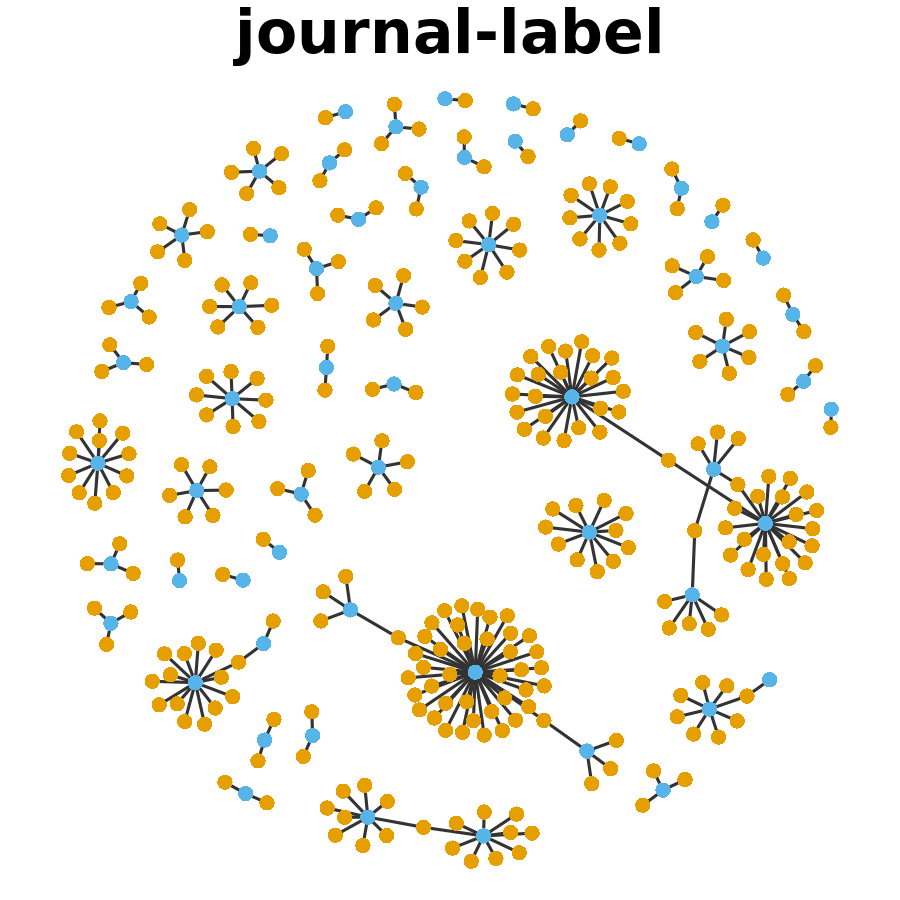
\includegraphics[width=0.33\linewidth]{ambrose_dissertation_files/figure-latex/mod-proj-1} 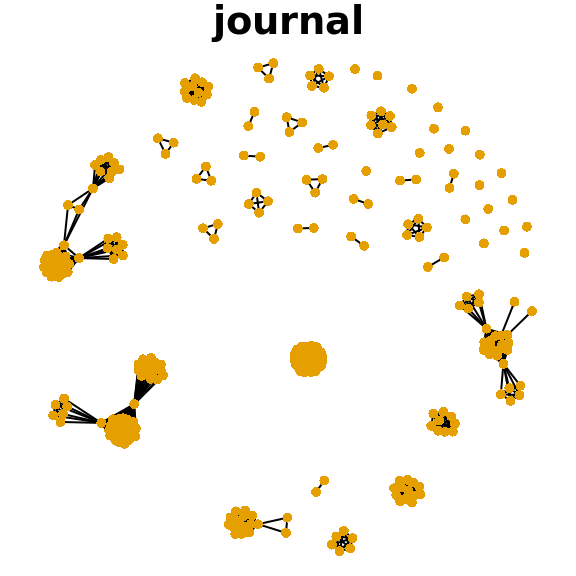
\includegraphics[width=0.33\linewidth]{ambrose_dissertation_files/figure-latex/mod-proj-2} 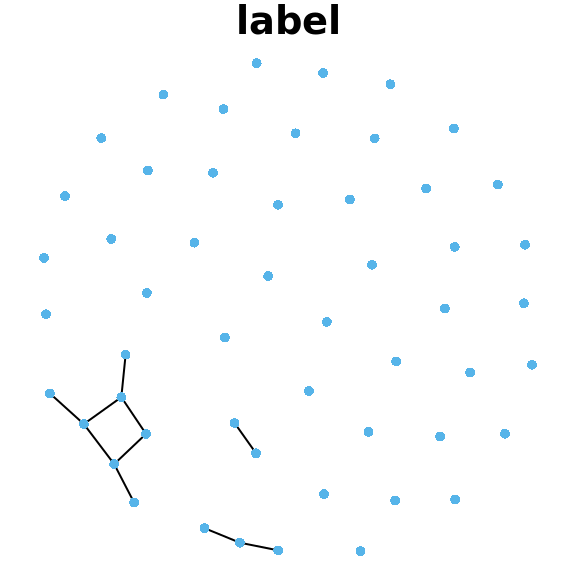
\includegraphics[width=0.33\linewidth]{ambrose_dissertation_files/figure-latex/mod-proj-3} 

}

\caption{Mode Conversion on a 300 Edge Random Sample of the JSTOR Title List Label Network}\label{fig:mod-proj}
\end{figure}

It is worth noting a few features of the unimodal projections or facets
illustrated in the second and third palens. First, unimodal projections
will always be made of up of overlapping cliques. Take the journal
facet; each journal bearing a particular label will be tied to each
other journal with the same label. Together they will form a clique, a
subnetwork of maximum density where all possible ties exist. Such
cliques grow nearly exponentially, as each additional journal with the
same label joins the clique and adds a number of ties equal to the
former size of the clique. In practice this means that very common
labels like ``Social Sciences'' can easily dominate the unimodal
projection of the network. Here the weighting of edges becomes
important; if two labels overlap because some nodes bear both labels,
then within the intersection of the two cliques the ties may be treated
as ``weighing more'' by adding the contribution of each label
separately. The exception is if the cliques overlap by only one node, in
which case they have a node but no ties in common. Nevertheless using
methods that take edge weights into account is a good way to ameliorate
the exponential influence of popular labels.

Second, though the unimodal facets of a bimodal network represent the
same data, each may have different characteristics especially in the
common case of a large population imbalance between modes. In the full
network we have 35 times as many journals as labels and each journal
sends multiple ties. This degree imbalance between the two modes may
mean that one facet is more dense than its inverse. Density is the
proportion of actual ties out of all possible ties. In Figure
\ref{fig:mod-proj} an imbalance may be observed where the journal facet
has many dense free floating or overlapping cliques and where the label
network appears to be mostly made of isolated labels save for the few
larger components. In the sampled network the journal facet is four
times more dense than the label facet. In the case of our full network,
the potential imbalance in degree distribution between facets happens to
be offset by the population imbalance itself. The densities in the full
journal and label facets are comparable, 26.2 and 27.3 percent
respectively, meaning that analysis will not merely hinge on which facet
is analyzed.

Third, unimodal projection has the effect of pruning what are sometimes
referred to as pendants, which are simply nodes with only a single tie.
. Each of the isolates in the label facet represents a larger or smaller
number of journals, which may be observed in the different sizes of the
free floating cliques of the journal facet, yet no matter their size
they supply no information about interdisciplinarity. Because the
journal facet captures both size (of cliques) and relatedness (clique
overlap) it is a better representation of the information of the
original bimodal network. Its drawback is that it is larger and more
unwieldy to analyze. The label facet offers a simpler picture of
interdisciplinarity.

\hypertarget{network-community-detection}{%
\section{Network Community
Detection}\label{network-community-detection}}

Each facet described above will help answer a different question about
disciplinarity in the JSTOR archive as indicated by JSTOR's labeling
policy. I aim to resolve the uncertainty about which labels count as
superdisciplines and to reveal patterns of sorting not apparent in the
labels themselves. The rationale for doing this is to observe not the
choices of JSTOR coders, but the tacit judgement they likely used in
applying labels. I expect that the 79 fine grained labels bely a simpler
classification scheme of academic genres.

I will use two techniques, community detection and graph visualization,
to answer these questions. Communities are really subnetworks of high
density, or clusters. I operationalize disciplinarity as the presence of
clusters within the journal facet network. Community detection on the
journal facet will answer how many superdisciplines there are and the
size of each in terms of the number of journals belonging to it.
Visualization of the label facet will show how hard or soft are the
boundaries between disciplines and where the strongest interdisciplinary
relationships lay.

First, I use community detection to partition the JSTOR journals into
mutually exclusive disciplines. Community detection is a set of network
methods designed to expose clusters by grouping nodes together such that
they send more ties to members of their own group than they send to
members of different groups. There is a cottage industry around
developing algorithms and statistical models to learn an unobserved
community structure of a network \citep[see][ for an excellent
review]{Fortunato2016Community}. The choice of the right community
detection method is controversial especially for very large networks in
which cross-validation is difficult. Fortunately the network at hand is
small enough to validate directly which lowers the risks of choosing the
wrong method .

To wit I adopt the well-known Louvain method of community detection
based on hierarchical modularity maximization. \citep{Blondel2008Fast}
Modularity is a quality metric quantifying the tradeoff between
within-group and between-group ties. The modularity of any given
partition of a network into clusters is equal to the proportion of ties
that fall within clusters minus the expected proportion of within-group
ties if ties were distributed randomly. A division that is as good as
chance would have a modularity value of zero, a division better than
chance a value between zero and one, and a division worse than chance a
value between negative one and zero. \citep[8]{Newman2004Finding} Higher
modularity scores indicate a better sorting of the network into densely
tied clusters.

The Louvain method is a bottom-up agglomerative algorithm. The procedure
starts by assigning each node to its own community. Then, for each node,
it assigns the node to the neighbor's group that would most improve
global modularity. It repeats this until no move improves modularity.
This forms the first layer in the hierarchy. It then collapses groups
into nodes and repeats the algorithm on the condensed network, stopping
at the first level where there is no modularity improving move to make.
The first layer represents the most local, the last layer the most
global resolution of community structure.

Modularity-based methods are tried and true, and their drawbacks are
well-known. The Louvain method is not deterministic, as the outcome may
(but usually does not) depend on the ordering of the nodes in the
reassignment qeue. However Louvain has several features that recommend
it. It is computationaly fast on small to medium graphs and it is freely
available in network analysis software. It also gives a hierarchical
solution that provides the analyst with options to inspect community
structure at a range of local and global resolutions, akin to a
cartography of counties versus one of continents. Given the small size
of our network, a local resolution will not be overwhelming, so Louvain
is preferable to other methods that only offer the coarser global view.

Table \ref{tab:jclu-tab-sup} summarizes the results of applying the
Louvain method to the journal facet and taking the most localized layer
of the community structure. Learned labels are applied to the clusters
by assigning each the name of its most frequent label. Community
detection sharpens the boundaries between fields by placing each journal
unambiguously in one superdiscipline or another. This mutual exclusivity
is apparent by the sum of the given labels exceeding 100\%.

\begin{table}[!htbp] \centering 
  \caption{JSTOR Journal Counts} 
  \label{tab:jclu-tab-sup} 
\begin{tabular}{@{\extracolsep{5pt}} lrrrr} 
\\[-1.8ex]\hline 
\hline \\[-1.8ex] 
Superdiscipline & Learned & Pct & Given & GPct \\ 
\hline \\[-1.8ex] 
Social Sciences & 790 & 28.9 & 916 & 33.5 \\ 
Humanities & 664 & 24.3 & 719 & 26.3 \\ 
Area Studies & 357 & 13 & 499 & 18.2 \\ 
Science \& Mathematics & 307 & 11.2 & 360 & 13.1 \\ 
Business \& Economics & 266 & 9.7 & 285 & 10.4 \\ 
Arts & 240 & 8.8 & 293 & 10.7 \\ 
Law & 84 & 3.1 & 132 & 4.8 \\ 
Medicine \& Allied Health & 30 & 1.1 & 52 & 1.9 \\ 
Total & 2738 & 100.1 & 3256 & 118.9 \\ 
\hline \\[-1.8ex] 
\end{tabular} 
\end{table}

The first finding is that of the 79 labels these eight form the top of a
hierarchy of superdisciplines. Area Studies stands apart and is not
subsumed under either Social Sciences or Humanities. Social Sciences
journals predominate due to JSTOR's initial focus in that area, even
without counting economics among them, and Science \& Mathematics counts
for a larger than one might think. Economics stands apart from the
Social Sciences, and indeed Business \& Economics marks the transition
from the larger academic journal space to the smaller professional space
of Arts, Law, and Medicine \& Allied Health.

The given labels do overlap and we can recover a picture of
interdisciplinary by clustering and visualizing the label facet. This
facet presents a simplified view. Recall that each facet represents the
same data, the difference being whether a journal or a label is
represented as a node or an edge, and that there is a population
imbalance in favor of journals over labels. The larger the population
the easier it is to partition into a greater number of subpopulations.
Converseley, because there are far fewer labels than journals, we would
expect the clustering to be less granular for the label network than for
the journal network. In fact there is only one less cluster--Law--which
is subsumed under Social Sciences.

\hypertarget{network-visualization}{%
\section{Network Visualization}\label{network-visualization}}

Figure \ref{fig:jclu-lnet} visualizations the relationships among
disciplines, where again the strength of ties is equal to the number of
journals bearing both labels. Here the label with highest number of ties
within its cluster becomes the category name of the cluster. That label
is then ommitted as a node and is instead visualized as a color coding
of its cluster, reflecting the special status of the superdiscipline
labels.

Unlike traditional graph visualizations that are designed to be pleasing
to the eye, this one is drawn according to a statistical model called a
latent position or latent space model. It starts with a simple idea that
the weight of the edges (the number of journals carrying both labels) is
a count that follows a Poisson distribution. This distribution may be
modeled by log-linear regression where the logarithm of the mean of the
distribution is a linear function of an intercept term and covariates.
What is interesting about the model is that the covariate of interest is
treated as the distance between the nodes in an unobserved or latent
space. The distance is treated as negative such that as nodes get closer
together (as the negative distance increases) the count of the edge
weight between them increases (technically the logarithm of the mean of
the count increases).

It is an elegant idea, but estimating the model is complicated. The
distances are metaphorical, and to realize them requires positing a
euclidean space in which each node has coordinates. From the coordinates
the distances can be easily caculated, but knowing which are the right
coordinates requires a complicated estimation routine based on
optimizing goodness of fit between guesses of the coordinates and the
actual count data. The estimator begins with coordinates taken from the
conventional Fruchterman Reingold layout algorithm and uses Markov Chain
Monte Carlo simulation to converge toward the positions that optimally
fit the latent space assumption \citep[See][ for details of the model,
estimation, and software]{Krivitsky2008Fitting}. Even if the estimator
does not arrive at a perfect solution it improves upon a conventional
layout in the direction of meaningful, and not just pretty, aesthetics
thereby helping the viewer to avoid artifacts and perceive real
information about the network.

Another great feature of the latent space model is that it allows
additional terms to be fit alongside the latent distances. It is
possible to control for or net out the effect of nuisance terms like any
other regression. As discussed above there is a concern about the undue
effect of popular labels. We have already tried to remove the
superdiscipline labels from the label network, preferring to represent
them as color coded categories rather than nodes. Popular labels may
still remain, however, and due to the exponential growth of ties during
downmode conversion even a handful of them will have a disproportionate
influence on the global layout of the graph.

This degree distortion can be controlled for by what is called a
sociality term, which can be thought of as a measure of a node's
popularity. A sociality term is a score for every node that if positive
means a node is more attractive and if negative means a node is actually
repulsive of ties. When viewing the positions of a latent space model
also fit with a sociality term, the space will measure relatedness
without the effects of popularity.

Figure \ref{fig:jclu-lnet} plots the results of a latent space model on
the label facet omitting superdiscipline nodes.

\begin{figure}

{\centering 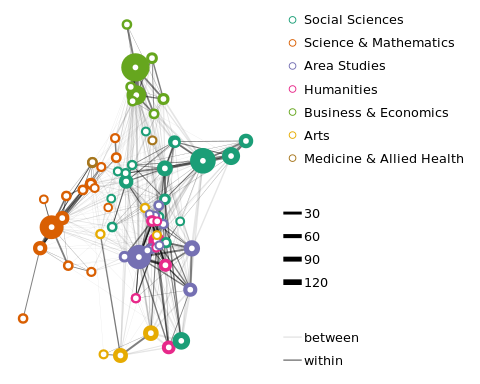
\includegraphics{ambrose_dissertation_files/figure-latex/jclu-lnet-1} 

}

\caption{Discipline Network in Latent Space. Node size represents sociality. The larger a node, the more attractive it is, and the larger a white dot within a node, the more repulsive it is.}\label{fig:jclu-lnet}
\end{figure}

Here some of the granular categories are collapsed. The humanities
includes arts, as we might expect, but also area studies, which one
might have classed with the social sciences, but which bear stronger
ties to cultural studies like music, folklore, religion, and language
and literature. Law and medicine and allied health are grouped with the
social sciences, and business and economics is maintained as separate
field due merely to the attachment of three professional
fields--development studies, management and organizational behavior, and
marketing and advertising--to their parent disciplines business and
economics (not to be confused with the separate and ommitted label
``business and economics''), which are themselves strongly tied to the
social sciences.

\begin{verbatim}
Setting the `off` event (i.e., 'plotly_doubleclick') to match the `on` event (i.e., 'plotly_click'). You can change this default via the `highlight()` function.
\end{verbatim}

\begin{figure}

{\centering \includegraphics{ambrose_dissertation_files/figure-latex/layouts-1} 

}

\caption{Fruchterman Reingold and Latent Space Layouts Compared}\label{fig:layouts}
\end{figure}

Though graph layouts are imperfect and should not be overinterpreted,
the global features of facing within clusters do indicate the
disciplines that straddle boundaries. On the border between the social
sciences and science and mathematics are the social sciences dealing
most with the physical problems of space, health, and technology. On the
edge of the humanities and social sciences are history, philosophy, and
anthropology.

\hypertarget{cit}{%
\chapter{The Social Science Citation Landscape, 1900-1940}\label{cit}}

\hypertarget{abstract-2}{%
\subsubsection*{Abstract}\label{abstract-2}}


Knowledge mapping of acadamic journals promotes the
conservation of intellectual history and stimulates discovery of
underexplored intellectual opportunities. Treated as a large network
community detection problem, I demonstrate how to apply the clique
percolation method to map two kinds of recorded knowledge: citations and
full text. The features of generated maps are explained, and
interpretive methods including visualization are presented. We use
American social science scholarship in the first third of the 20th
century prior to U.S. entry into World War II as a case, and describe
how the intellectual landscape of four separate social science
disciplines developed.

\hypertarget{keywords-2}{%
\subsubsection*{Keywords}\label{keywords-2}}


citations, k-clique communities, community detection,
landscape

\hypertarget{introduction-1}{%
\section{Introduction}\label{introduction-1}}

If knowledge is power then scholar must be a powerful class. But what
kind of power is knowledge and in what way do scholars wield it? Is
knowledge powerful a utility, like water or electricity, to drive a tool
and accomplish a task? Is it an asymmetry of information, like a stock
tip or the combination to a safe, that gives one a leg up on her
competition? Is knowledge like the power of an authority, like a
governor, a military commander, or clergyman, to compel the loyalty and
obedience of another person?

How we conceive of knowledge affects how we view the nature and
importance of the people and institutions that produce it. Scholars
certainly do not have a monopoly on the utilization of production of
knowledge in society, but their occupational roles are conditioned by
the stuff of knowledge at the same time that knowledge is itself
conditioned by the technology and social arrangements that constitute
scholarly occupations.

\hypertarget{scholarly-communication-vs-knowledge-terrain}{%
\subsection{Scholarly Communication vs Knowledge
Terrain}\label{scholarly-communication-vs-knowledge-terrain}}

If the production of culture perspective were to argue against Marx's
German Ideology, it might say, ``Not all mental laborers have soft
hands.'' Marx drew a course distinction between mental and material
labor to demonstrate that the former is not possible without the latter,
even when at the time mental labor had already been commidified with the
advent of print media. The production of culture perspective simply
effaces the distinction altogether; mental labor, or cultural products,
are like any other industrialized commodity.

The production of culture perspective is at odds with public sector
economics that argues that non market mechanisms create value where
markets fail to do so. \citep{Hayes2000Assessing}

Remuneration

Are culturally interior products referenced by socially superior
producers?

\hypertarget{wok}{%
\subsection{Mapping Knowledge Terrain}\label{wok}}

\hypertarget{knowledge-stuff}{%
\subsubsection{knowledge stuff}\label{knowledge-stuff}}

There are two reasons to map knowledge spaces. First, we may want to
know how knowledge develops as a resource unto itself. Second, we may
want to exploit such a map for a productive purpose. Here we will
attempt the second as prologue to the first. We will tackle the
technical problems of constructing a map. We will show how a map can be
put to use. Finally, we will investigate how the particular map we make
may tend to predictably get us lost.

All knowledge mapping requires first an ontological and then an
analytical action. Ontological actions delineate the things that matter.
They arbitrarily construct from perception the items that we then think
about. While onotological decisions tend to define the scope of
everything that may be learned from an investigation, they are often
assumed rather than demonstrated. Actor Network Theory (ANT) provides a
unique example of a method of research that, because it is ethnographic
and thus marinating in an abundance of perception, allows the cast of
ontic characters to grow. Literally anything can be deigned significant
for inclusion in a web of knoweldge. In an ANT study of science, if the
feel of a reading chair modifies a reader's oreintation to a text they
are reading, the chair counts.

The lion's share of knowledge mapping studies are not so ontologically
radical as ANT. Take the field of bibliometrics. The ontological
decision here is to take documents as the primary ontic. Documents are
nothing but collections of glyphs, so the first task of bibliometricians
tends to be to map glyphs to terms and analyze them. Here we have
already used the ontic triad underlying bibliometrics. In the sentence

\begin{quote}
``Go, dog, go!''
\end{quote}

there are twelve discrete glyphs and two terms. A grammatical cutting
rule renders the glyph sequences as

\begin{quote}
``Go,'' ``dog,'' ``go!''
\end{quote}

and a tokenization rule maps the cuts to two terms

\begin{quote}
``go'' ``dog'' ``go''
\end{quote}

which may in turn be analyzed, for instance by counting the tokens. The
documents form the bins within and across which the terms will be
analyzed. The token, as a mere operational step, is used and then
dispensed with unless questions of measurement surface. Clearly the
\emph{glyph-term-document} (GTD) ontic does not care about the armchair
of a reader of a document, and indeed does not even care about the
reader herself.

So the reader is invisible because she is not inscribed in the document.
What about the writer? Bibliometricians may backfill GTD by entity
recognition or grounding. Once terms are recognized, we may further
recognize that we know more about them. A simple example of this is
pulling out ``metadata'', for instance, the author of a document. The
author's name is not just any term, but a conceptually very important
one. Grounding is how bibliometrics may be linked to theories and
programs of greater importance.

Bibliometrics has indeed been based more on the reference of a text as a
particular grounded entity rather than on the use of the full text of a
document. If a text is a building, the reference is its address. More
precise than a name, an address is a codification of different
hierarchically ordered elements that describe the location of an entity.
The consistent tokenization of a reference is not an easy task, as it
depends on entity recognition of several different kinds of things,
including year of publication, author, title, and source.

The citation became the basis of the concept of a web of knowledge as
coined in the work of Eugene Garfield and institutionalized in the
Institute for Scientific Information (ISI).

Citations solved the problem that ideas do not have signatures or
addresses that we can trace reliably. Jargon is an attempt to give an
idea a unique address as an idiosyncratic term, and etymology seeks to
hierarchically order words according to their origins, but an idea per
se will always elude precise identification. Unlike a document, an idea
is not mechanically reproducible; it always requires interpretation and
understanding in a mind, and a mental event as subtle as an idea cannot
be observed.

\citep{Lederberg2000How} Garfield conflates citations with several roles
in the network around ideas. Compares value of citations to value of
subject coders, coding meaning of paragraphs intractable. ISI became a
commercial pursuit because Garfield failed to get scientific
institutions, especially the NSF, to fund it. The goal was primarily
practical, to give researches access to current or historical references
relevant to articles, perhaps especially their own, they knew they were
already interested in.

Unlike ideas, documents are physical artifacts and can be traced
empirically. They are fungible, reproducible, and locatable with
addresses.

The reproduction and location of ideas cannot be reliably observed, and
documents only contain ideas in a metaphorical sense, as a Leyden jar
was once thought to contain electricity.

Documents are the tangible and fungible currency with which scholars
communicate about ideas, yet how knowledge is actually communicated via
documents is not amenable to direct observation at scale. In
bibliometrics they have served as a proxy for ideas.

There have been two main orientations to mapping the web of knowledge,
description and conscription. Description has either scientific aims, to
underatand and explain the facts of knoweldge development, or practical
aims, to locate and retrieve knowledge required for a particular
purpose. Conscription on the other hand aims to mobilize bibliometric
patterns of knowledge as measures of value in competitive markets,
namely hiring, promotion, and awards within scholarly professions.

There are several ways to digitally represent texts as knowledge.

From an empirical perspective, texts are nothing but collections or bins
of glyphs. The current paradigm is to render glyphs and recognize them
as terms. Such terms may then be analyzed, for instance, by counting
diction. Alternative paradigms are cropping up

Second is entity recognition or grounding, where recognized terms are
mapped to an existing database of structured knowledge.

\citep{Pilkington2009evolution}

\hypertarget{disciplines-as-a-large-world-co-reference-network}{%
\subsection{Disciplines as a Large World Co-reference
Network}\label{disciplines-as-a-large-world-co-reference-network}}

A large world network is not amenable to traditional visual
representations due to its extreme density. Scholars often use edge
filtering to reduce this density down to a manageable size for
vizualization. Unfortunately this convenience function renders a large
world as a small world and grossly misrepresents the true structure of
the network. In the KCC representation, the network is partitioned into
subnetworks of differential density. Nodes are included in a subnetwork
if they are involved in ties at a given floor of density, for instance,
they need to be tied to at least five other nodes. At a level of five,
then, nodes involved in only four ties would be excluded. As this
standard is raised, more nodes are excluded. This results in a nested
set of subnetworks, where nodes included in a community at a lower
threshold are excluded at a higher threshold. Subnetworks of lower
density thresholds are always as big or larger than those at higher
threshholds. Moreover, higher density subnetworks are always subsets of
lower density communities, as their density meets and exceeds the
standard for inclusion at the lower level. As one can imagine, inclusive
levels are larger. As the threshold is raised subgroupings are sluffed
off until reaching points of maximal density. In a world where almost
everything is connected, there are no structural holes to reveal
differences between subnetworks. Instead, we can view the structure as
gradations in density within a very densely connected world.

Nodes meeting the highest standards can be thought of as omnivorous;
their ties draw them to the masses, but the masses are not sufficiently
tied to the higher standard community. Where the gentry may be as
comfortable at the movies as at the symphony, the layity lacks access to
the more erudite circles.

What is the credential that would allow a node to climb the hierarchy?
One's list of aqcuaintances must overlap by a certain amount (defined by
the threshold) with the membership of the higher tier. Indeed their
inclusion would change the credentials of everyone they are tied with,
as anyone who was just under the standard would be tipped in based on
their friend's promotion.

In the KCC model the references are the members of the hierarchy. Their
association with each other is determined by how they are used by
published authors. Authors who include two references on their
bibliography tie those references together in the network. Indeed each
citing article lays down a dense clique of references, and the impact of
an article grows quadratically with the length of its reference list.

\hypertarget{methods}{%
\section{Methods}\label{methods}}

\hypertarget{data-1}{%
\section{Data}\label{data-1}}

\hypertarget{results}{%
\section{Results}\label{results}}

The structure of a large world as revealed by KCC can be explored in a
bottom-up and top-down fashion. Bottom-up observes 3-clique communities
first. In the social science co-reference network.

\begin{figure}

{\centering 
\includegraphics{ambrose_dissertation_files/figure-latex/kcc2tree-1} 

}

\caption{K-clique Community Structure ([popout](tree.html))}\label{fig:kcc2tree}
\end{figure}

Figure \ref{fig:kcc2tree} shows a KCC model of the social sciences in
the first half of the twentieth century.

Disciplinarity and interdisciplinarity are revealed in a novel fashion
in the KCC model. Disciplinarity is shown as a level of exclusion.

\hypertarget{continents}{%
\subsection{Continents}\label{continents}}

The global map is made of many separate regions ranging in scale from
large continents to small isles. These regions are either shawlowly
connected or entirely separated from each other. The vast majority of
these regions are ``flat isles'' with little to no internal structure of
their own. Most flat isles are supported by only a single article, some
by a couple of articles penned by the same author, and only a few
represent real activity among a small group of different authors.

\begin{figure}

{\centering 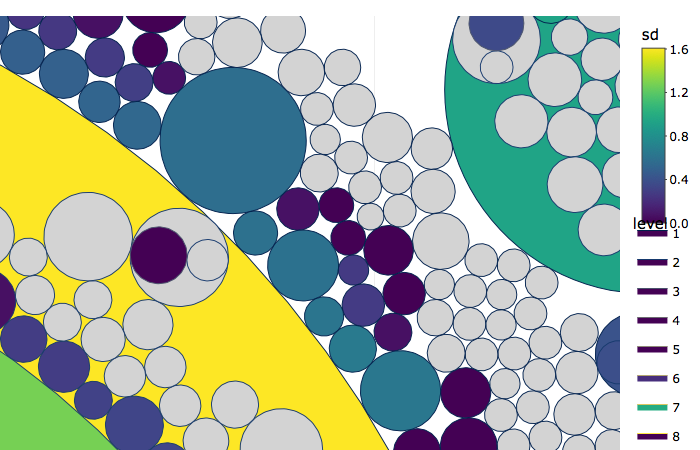
\includegraphics[width=9.72in]{img/flat-isle} 

}

\caption{Flat Isles, where Reviewers tend their Flock}\label{fig:flat-isle}
\end{figure}

The most substantial flat isle , the largest unenclosed and unenclosing
circle in Figure \ref{fig:flat-isle}, comes from four authors publishing
in the same 1930 \href{https://www.jstor.org/stable/i40084238}{issue} of
\emph{Zeitschrift Fur Nationalokonomie}. It includes 50 references the
most prominent of which are Angell's 1926 \emph{The Theory of
International Prices} and Tugwell's 1924 \emph{The Trends of Economics}.
The structure of the group is provided entirely by an article by Robert
Reisch ; the other three shared no references in common and Reisch's
article, titled ``The `Deposit'-Myth In Banking Theory'' and containing
108 references, is likely to have been written as an introduction to the
journal on the basis of what had already been accepted for publication.

Another flat isle of four articles has the exact same pattern, also from
\emph{Zeitschrift Fur Nationalokonomie} but from an
\href{https://www.jstor.org/stable/i40084262}{issue} in 1937, the
article on the first page of the issue, titled ``Theory Of Capital,
Introduction'' by von Hayek and containing 25 references, includes
subsections of the bibliographies of three other articles that do not
themselves overlap. Normally the longer a bibliography the more likely
it is that an article functions as a review linking other disparate
bibliographies. That von Hayek's article has such a short bibliography
and yet still links three otherwise separate articles confirms its
derivative character.

The following features then suggest when a flat isle represents an issue
introduction. All articles are published in the same issue. The removal
of the longest bibliography in the community yields a network of
disconnected components each uniquely representing the remaining bibs.
This longest bib is also either the first article in the issue or
precedes the others in pagination. These characteristics suggest
authorship internal to the editorial process itself. Later we will
explore how the removal of such articles helps to reveal ``bottom-up''
structure by removing the editorial advantage of certain authors to
bestow an ad hoc intellectual coherence on scholarship.

Table \ref{tab:iss-int} enumerates issue introductions and shows how
many are the structuring article in their community.

\begin{figure}

{\centering 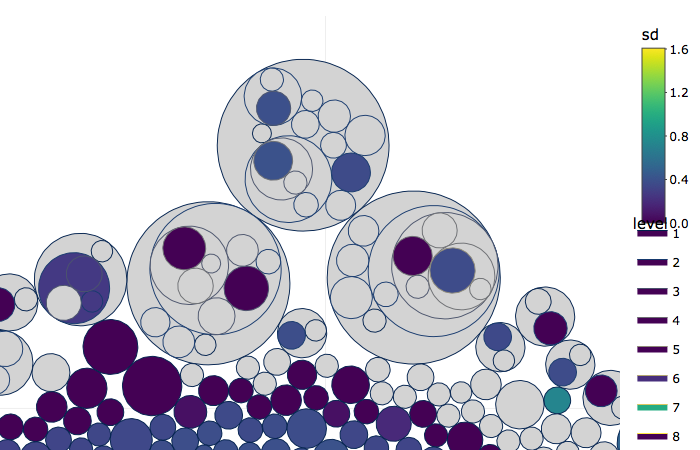
\includegraphics[width=9.72in]{img/hill-isle} 

}

\caption{Hill Isles, where the Wild Things Are}\label{fig:hill-isle}
\end{figure}

Reviews, whether they are self described as such, borrow directly from
the bibliographies of one or more seed articles, and in this way they
contribute a disproportionate amount of the global structure of the
co-reference network. This kind of review, rather than looking again at
an existing intellectual trend, creates the cohesion it purports to
describe. Flat isles, especially if they are large, are flat due to the
retrospection of a usually solitary reviewer. Compare this to ``hill
isles'' with more internal structure growing out of the related but
uncoordinated reference activity of authors.

\begin{figure}

{\centering \includegraphics{ambrose_dissertation_files/figure-latex/k3c1-22-1} 

}

\caption{Hill Isle in Graph Layout}\label{fig:k3c1-22}
\end{figure}

\hypertarget{peaks}{%
\subsection{Peaks}\label{peaks}}

The KCC model reveals

\hypertarget{valleys}{%
\subsection{Valleys}\label{valleys}}

\hypertarget{do-reference-lists-describe-author-knowledge}{%
\subsection{Do reference lists describe author
knowledge?}\label{do-reference-lists-describe-author-knowledge}}

The peer review process can now be thought of as a process of auditing
credentials. An author makes an opening bid with the submission of a
particular reference list. What this reference list implies about what
the author knows is unclear. One may omit a knowledge signal because it
is truthfully irrelevent or in a deceptive sin of ommission oriented to
what they expect to be the expectations of editors and reviewers. One
may also include what they do not know out of error, bragadoccio,
carelessness, or fraud. Part of the work of reviewers will be to
validate those claims to knowledge.

\hypertarget{voc}{%
\chapter{Vocabularies of Anthropology and Sociology,
1888-1922}\label{voc}}

\hypertarget{abstract-3}{%
\subsubsection*{Abstract}\label{abstract-3}}


Knowledge development of journals in sociology and
anthropology is measured as the change in topic prevalence over time.

\hypertarget{keywords-3}{%
\subsubsection*{Keywords}\label{keywords-3}}


sociology of knowledge, topic modeling, history of social
science

\hypertarget{kd}{%
\section{Knowledge Development}\label{kd}}

What were the ideas that predominated in the social sciences at their
formation as professions in the postbellum United States? What was the
course of their development over a generation of scholarship? In this
study I will answer these questions inductively through a reading of the
original journals in each discipline. Though the goal is substantive,
the methodological challenges of consuming a large quantity of text will
feature importantly in the story that unfolds. Along the way I will
demonstrate the usefulness of the computational \emph{distant reading}
that is being explored in the humanities and how it can be combined with
traditional textual analysis for social science purposes. While
controversial in humanistic circles that emphasize the primacy of the
reader's novel interpretive work when consuming text, distant reading
fits comfortably within a social science epistemology that aims to
achieve an objective description of intellectual history Indeed,
computational methods offer a useful backstop to the idiosyncrasy of a
particular person's reading of history.

Computational textual analysis promises to automate a particular slice
of what hermeneutic methods accomplish. Hermeneutics claims that through
historical methods it is possible to reconstruct the interpretive
context of texts such that they can be understood in the same way that
contemporary historical actors understood them. Establishing such
context is a laudable yet arduous feat of historical research to uncover
the social and intellectual milieu of a particular text. This is the
gold standard approach, but one that restricts the field to specialists
with the training and resources necessary for the undertaking.

Computers cannot study history in this way. What they can do, however,
is mine source material for limited kinds of contexts. The kind I am
concerned with below are the \emph{historical vocabularies} that writers
used to construct texts in historical time. Vocabularies are glyphs
without grammar; they do not mean anything, but nothing meaningful can
be said without them in the present or in the past. They are the
mediated form of language, and in communicating with each other
historical actors leave traces that survive perfectly in time so long as
texts themselves survive.

While computers cannot read meaning in texts, and can barely recognize
it, they are almost as good as humans at recognizing the glyphs of
texts, and vocabularies are nothing but glyphs. What computers lack in
smarts, they make up in speed and memory. The quantitative scale of
their recognition makes for a qualitative shift because vocabularies can
be enumerated across immense corpora of texts. Immense, at least, by
human standards as there are limits to even computer memory and speed.
Yet such enumeration of texts into objective historical categories; this
is a profound resource for the intellectual historian. That one could
begin a reading with such context would be a transformative research
tool. Vocabulary enumeration, by which I mean simply the counting and
classifying of texts according to the vocabularies they contain, invites
a population studies approach to intellectual history. Where
sense-making is driven by comparisons, a reader's arbitrary combination
of texts is guaranteed to lead to anachronism. But if we can know that
texts are relevant to each other without knowing why, we have done some
small amount of hermeneutic work by supplying texts as historically
correct context to each other.

And even going so far as abandoning the project of reading texts in a
historically correct way, vocabulary enumeration can still lend
objectivity to a novel construction, a productive anachronism, of
textual meaning. Because vocabularies, the problems solved by computers,
are mathematically, algorithmically, or stochastically determined, they
may provide an immutable description of corpora that, like a map,
enables individual and collective exploration within a common framework.
Such maps may become the parameters of interpretive methods, which we
may use to surface and control some of our subjectivity.

This at least is the rationale for what follows. I begin with a
discussion of intellectual history of two social sciences, anthropology
and sociology, in the United States. I take a coarse view of national
history as the history of wars because of their downstream effects on
government activity and institutional investments. The first period is
between the end of the American Revolution (1783) and the end of the
American Civil War (1865) and is the national context for the origin of
U.S. anthropology. The second period is after the Civil War until the
end of World War I (1918) and is the context for the origin of U.S.
sociology and of modern U.S. higher education generally. Wars of
territorial expansion are waged regularly during both periods against
native peoples and rival colonial empires, and social research was
always recruited to solve attendant problems of population and to
provide rationales for the relationships with and understandings of
conquered or would-be conquered people.

I use intellectual histories of anthropology to characterize the
antebellum period, and the same for the postbellum period including
sociology. The most important journals in each field date from the
postbellum period, and the appearance of each is implicated in the
project of professionalization for each discipline. The 1920s marked the
end of war with the last of the militating American Indian tribes, and a
reckoning with the darkest sides of industrialization laid bare by WWI.
Social research had by this time completed a shift from colonial to
industrial problems and enjoyed a golden decade of development as a
profession, punctuated by the next great historical crisis in the Great
Depression. With the 1920s begins the adolescence of social research,
which is beyond the present scope. This study is of its childhood, which
ends with the Great War. I however draw the study out until 1922 because
it is the end of the public domain in U.S. copyright, to aid in the
reproducibility of the analysis and so that all readers may recover the
texts in question without difficulty.

\hypertarget{kd-dq2}{%
\section{Social Science Journals}\label{kd-dq2}}

The journals within social science cover five different subdisciplines.

\begin{table}[!htbp] \centering 
  \caption{JSTOR Social Sciences Journal Counts} 
  \label{tab:jclu-tab-sub} 
\begin{tabular}{@{\extracolsep{5pt}} lrrrr} 
\\[-1.8ex]\hline 
\hline \\[-1.8ex] 
Subdiscipline & N & Pct & Labeled & LPct \\ 
\hline \\[-1.8ex] 
Archaeology & 256 & 27.9 & 115 & 12.6 \\ 
Political Science & 219 & 23.9 & 183 & 20 \\ 
Education & 192 & 21 & 170 & 18.6 \\ 
Sociology & 160 & 17.5 & 145 & 15.8 \\ 
Anthropology & 46 & 5 & 89 & 9.7 \\ 
Population Studies & 22 & 2.4 & 27 & 2.9 \\ 
Geography & 18 & 2 & 32 & 3.5 \\ 
Transportation Studies & 3 & 0.3 & 7 & 0.8 \\ 
Total & 916 & 100 & 768 & 83.8 \\ 
\hline \\[-1.8ex] 
\end{tabular} 
\end{table}

\begin{figure}

{\centering 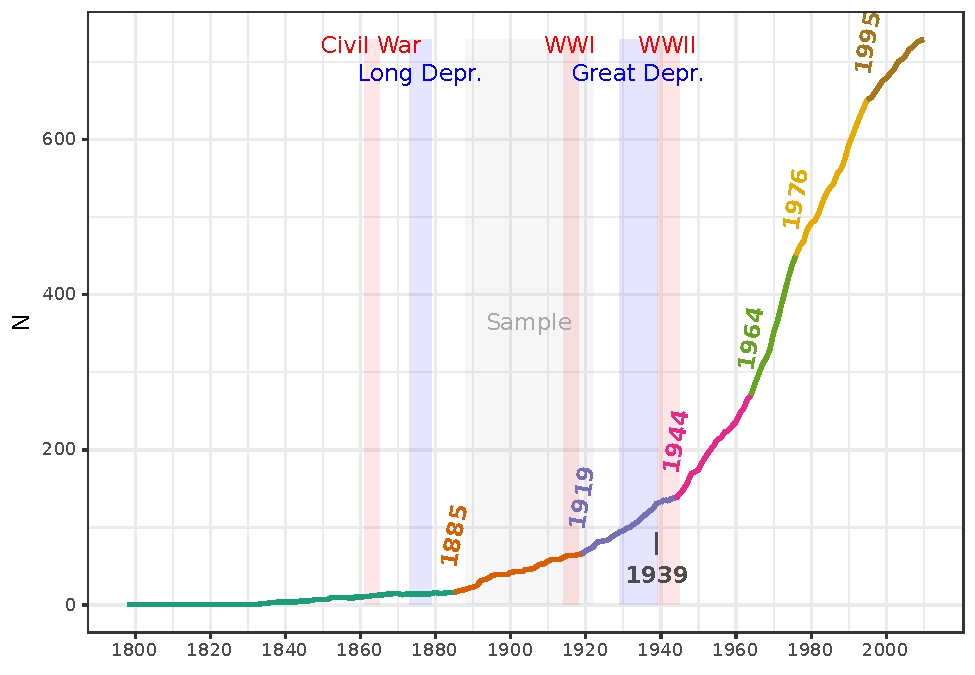
\includegraphics{ambrose_dissertation_files/figure-latex/jstorm2fig-1} 

}

\caption{Periods in the Growth of the Number of Social Science Journals in the JSTOR Archive}\label{fig:jstorm2fig}
\end{figure}

\begin{figure}

{\centering 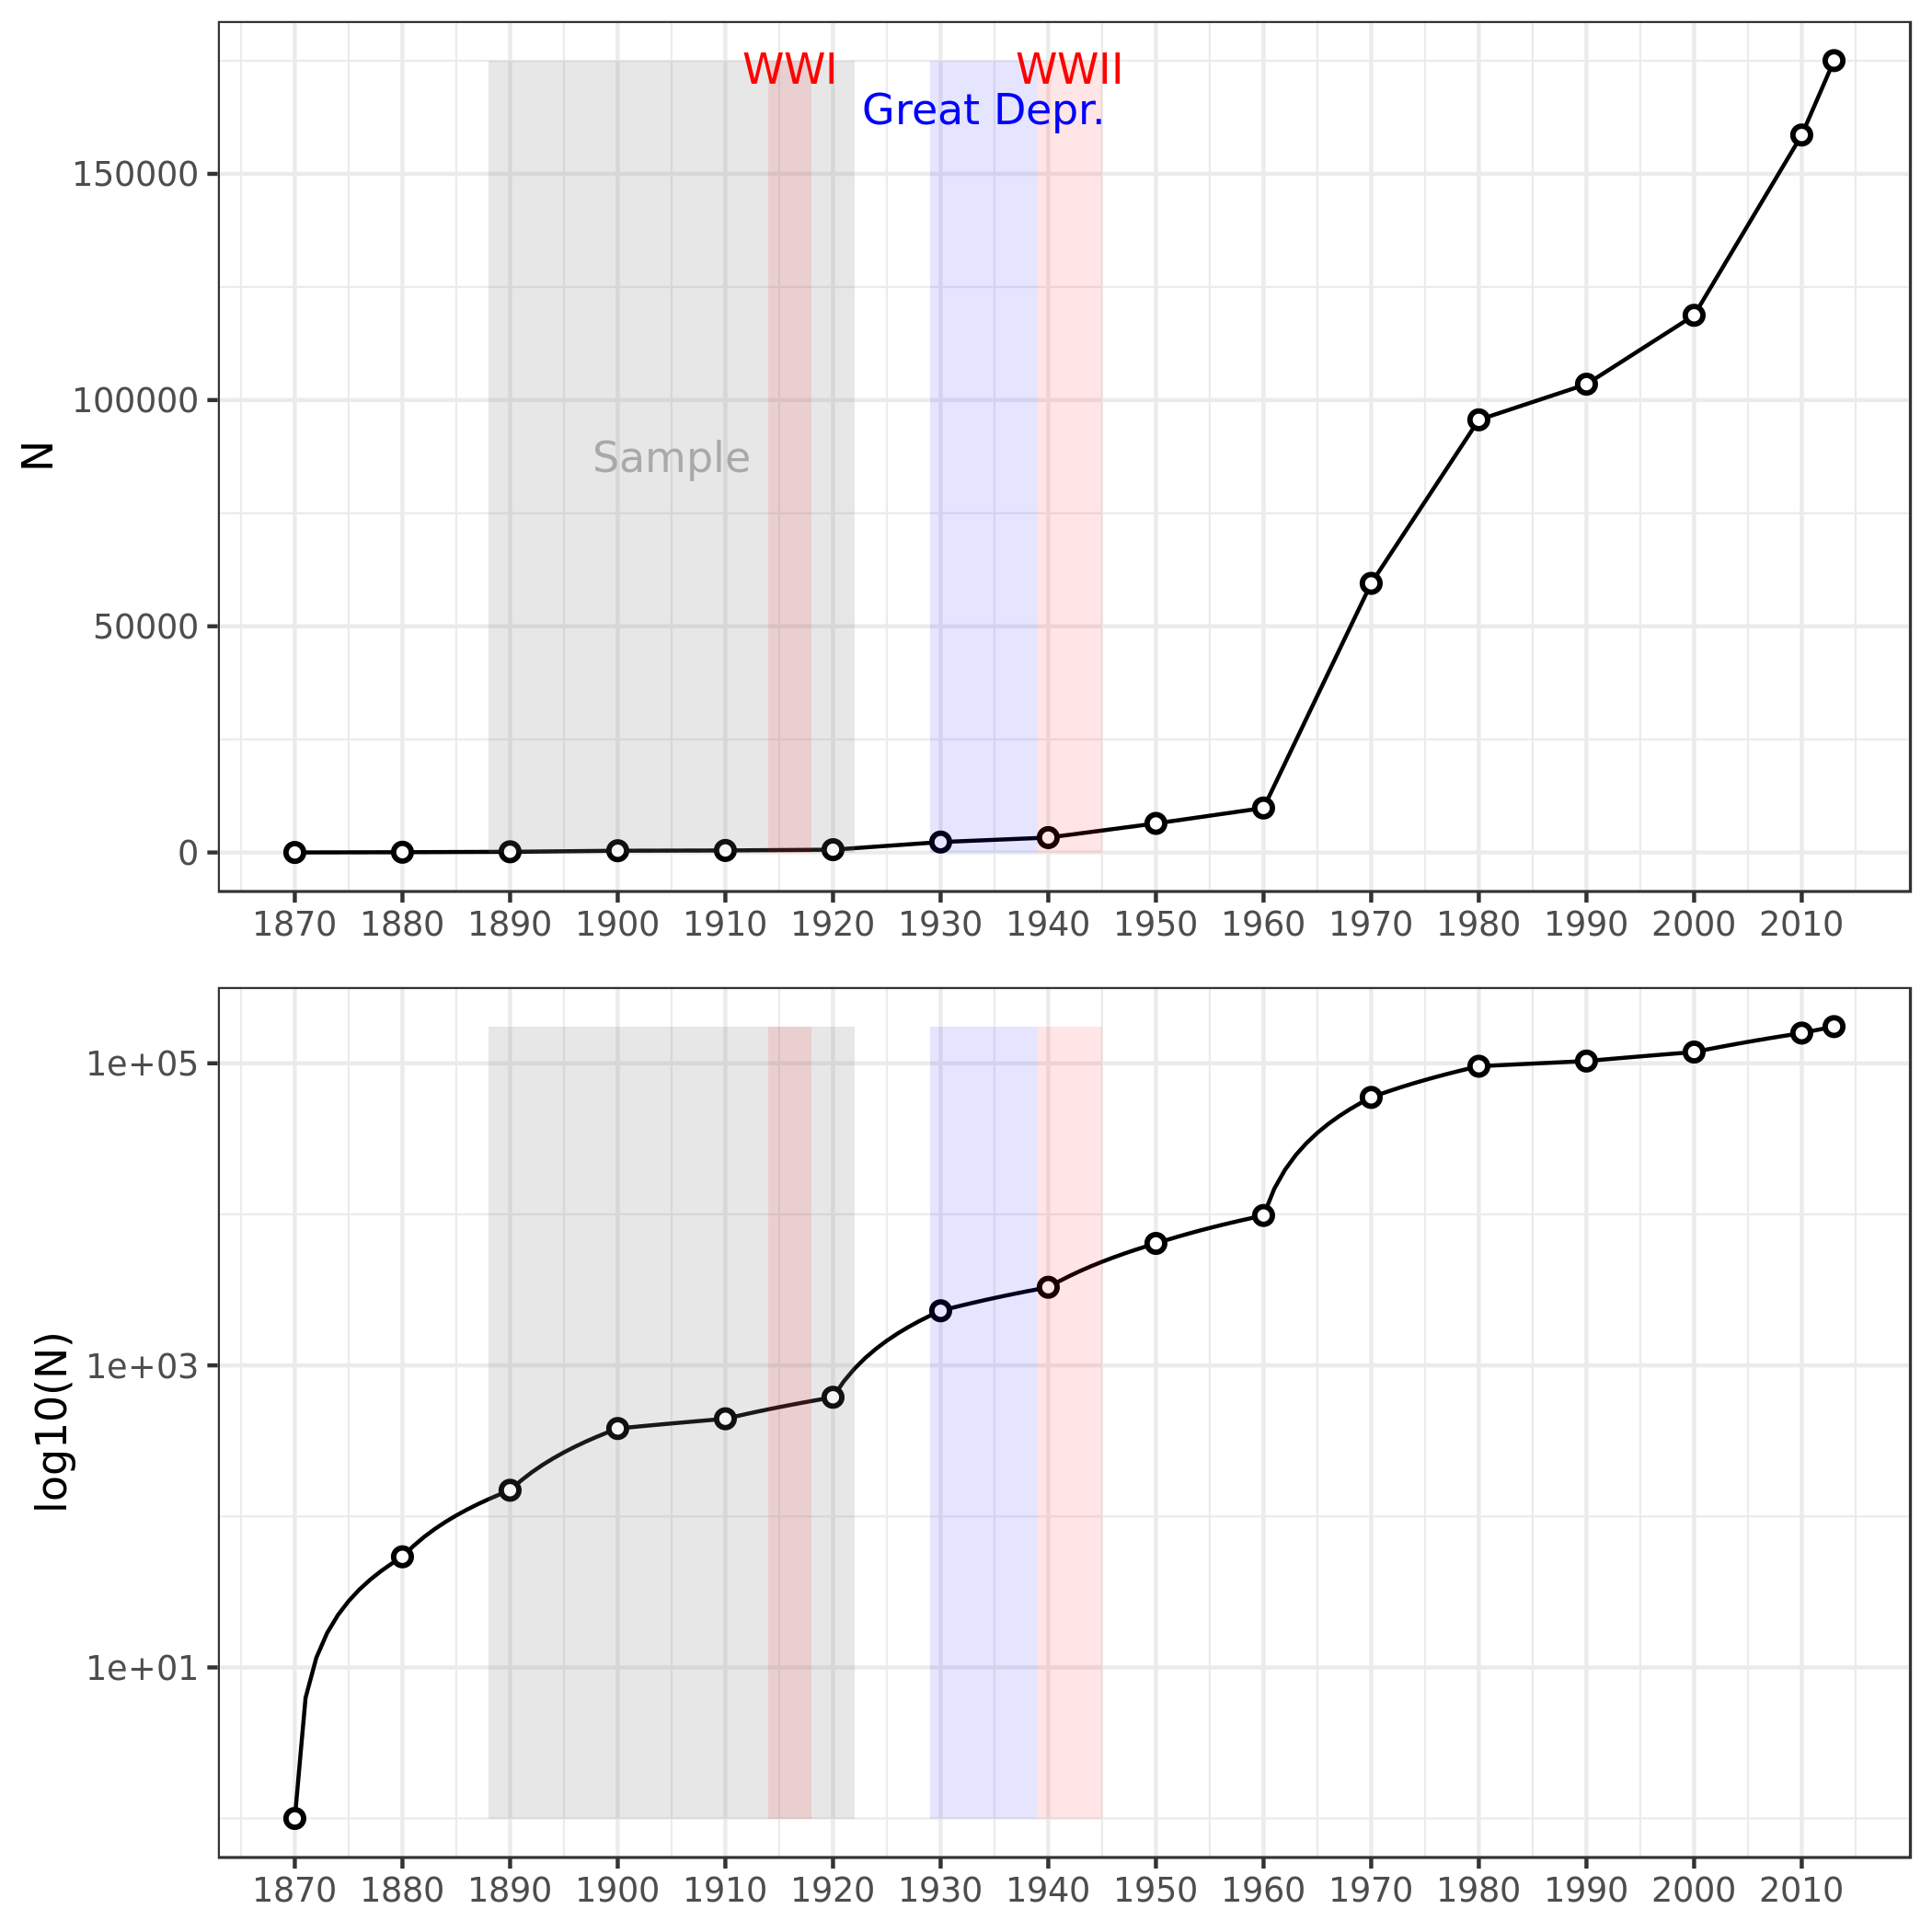
\includegraphics{ambrose_dissertation_files/figure-latex/nces2phd-1} 

}

\caption{Decennial growth in number of PhD degrees conferred in the U.S.}\label{fig:nces2phd}
\end{figure}

\begin{figure}

{\centering 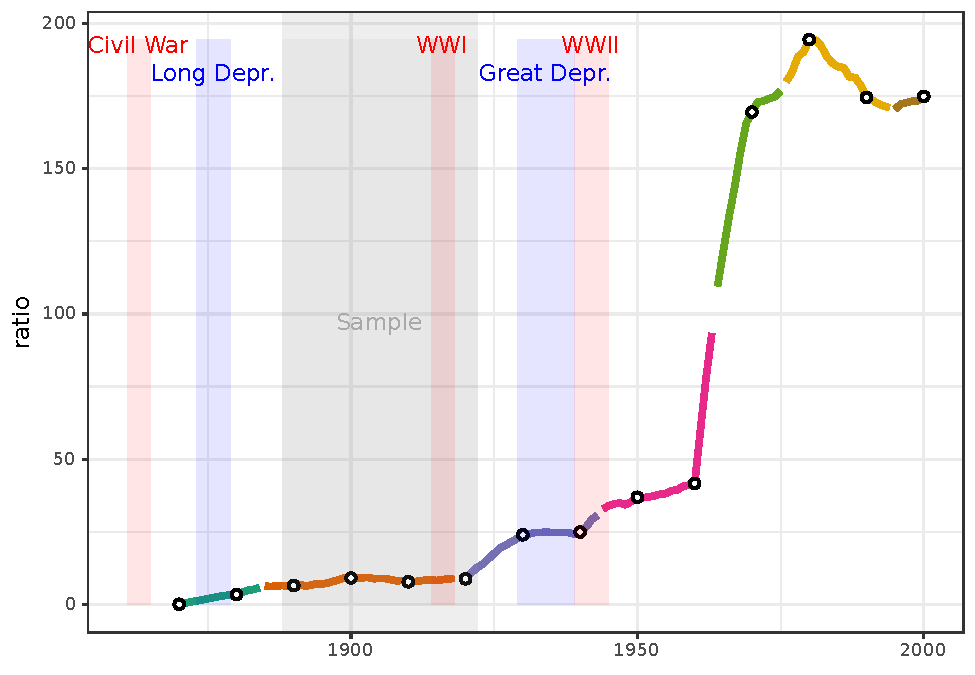
\includegraphics{ambrose_dissertation_files/figure-latex/nces/jstorm-1} 

}

\caption{Number of PhDs conferred in the United States per Social Science Journal}\label{fig:nces/jstorm}
\end{figure}

This period represents one of stable growth, as the size of the field
grows with the number of players on it. Between 1888 and 1922 there
tended to be about seven new PhDs in the U.S. for every social science
journal even as each population grew year over year. These growth
patterns begin to diverge around 1920 as a decades long acceleration of
personnel begins, relatively slowly between 1920 and 1960 at an average
acceleration rate of 22 PhDs per journal per year, and then quite
precipitously in the 1960s at an average acceleration rate of 121.

\hypertarget{topics-ideas}{%
\section{\texorpdfstring{Topics \normalfont{≟}
Ideas}{Topics  Ideas}}\label{topics-ideas}}

The strategy of the study occurs in four steps.

\begin{enumerate}
\def\labelenumi{\arabic{enumi}.}
\tightlist
\item
  Sort text into categories of similar vocabulary.
\item
  Describe the vocabularies that define category membership.
\item
  Describe vocabulary prevalence across time and discipline.
\item
  Validate category contents by a traditional qualitative reading of
  texts.
\end{enumerate}

I will spend considerable effort on solving the problem presented by
step 1, as here everything depends on the computational methods
employed. Steps 2 and 3 are straightforward given a successful
mathematical model of texts. Step 4 is seldom attempted, and may be the
hardest of all, because it is here that machine and human learning must
be integrated. If I am successful, if through these steps I may
operationalize the notion of cultural meaning or cultural logic as
conformity to vocabularies, then I believe a new horizon of intellectual
scholarship is possible. If on the other hand I find that
machine-learned vocabularies do not correspond to human-learned
understandings of the texts drawing on those vocabularies, then the
discovery will be negative, that distant reading is not a scientific,
historical, or hermeneutic method, but rather a toy at worst and a best
new humanistic method of reading texts de novo.

The mathematical tool I will rely on in step 1 is called topic modeling,
which refers to a variety of computational approaches to text data that
blur the distinction between qualitative and quantitative analysis. The
topic model paints a lexicographic picture of texts, analogous to the
demographic picture gained by a civil census survey of cities and towns.
To a topic model, texts are merely collections of terms (usually words)
that are counted to create the so-called ``bag of words'' description of
a text. In the same way that a census reduces communities to counts of
the names of people who live in them, topic modeling reduces texts to
the frequency of word choices in texts, to their diction or vocabulary.
Just as a census of people fails to capture the nuanced interactivity of
human settlements found in their culture, politics, and economic
activity, the topic model washes away the meanings and intentions behind
the words that are enumerated.

A population census would not be very helpful were it only a count of
the names of respondents, and of course the really helpful data derive
from the demographic and economic survey attached to the name. Text data
do not usually come with such a collection of rich covariates, yet
nevertheless topic models promise to discern helpful patterns from
counts alone. The trick behind the estimation of a topic model is that
it attempts to learn the demographic information (topics) without
asking, by merely looking at how the names alone (terms) are distributed
across geographies of interest (texts). If it can keep its promise, a
topic model applied to census data might recover the cultural patterns
latent in the distribution of names. It might, for instance, learn
different groupings of names that in turn correspond to markers like
age, race, national origin, or gender, so long as membership in those
categories was related to geography. It might, for instance,
successfully separate a category of Hmong names out from among the names
of all people living in St.~Paul because the non-Hmong names appeared in
other regions where no Hmong names appeared.

To call the category of names ``Hmong'' requires an interpretation of
the model, which by itself is just lists of names. This is the work of
step 2, and requires a little bit of shoe leather by trying to make
sense of what a list of names refers to. Here reading texts is like a
census taker knocking on a door, and a topic model's latent analysis
saves on this effort. Sometimes bringing domain knowledge to bear on the
list itself will suggest a category label, but often choosing a small
sample of texts as exemplars of the category. Still this requires much
less shoe leather than a traditional qualitative analysis in which each
text is studied directly. Of course the census is much more informative
because it asks about demographic categories directly thereby avoiding
the need for a latent analysis. In domains where rich covariates are not
yet available or are prohibitively expensive to acquire, latent analysis
provides promising clues of patterns that already exist. What is even
more interesting, and something that might surprise even census
analysts, is when latent categories do not correspond to known survey
items. In either event the power of topic modeling for inductive
analysis is to reveal structure in how names hang together that was
hidden.

Even without conducting the second labeling step, in step 3 it will
already be possible from the output of the model to inspect the
distribution of topics across available covariates, especially time.
These are the patterns that will help validate the topic models against
what is already known about intellectual history. For instance, the
power of institutional and generational change may well be apparent in
the historical distribution of topics. This step leads naturally into
step 4 by suggesting anomalies that can only be explained by a closer
look at the texts, the chore that the entire preceding analysis punts
on. In step 4 we learn either that our understanding of history was
wrong, or that our topic model was wrong, and there may be no method
other than one's judgement to decide.

In the next section, before we delve into the statistical and
computational nuances of topic models, I will spend some time developing
a few themes to help organize the blending of quantitative and
qualitative methods invited by topic modeling in particular and
computational text analysis generally.

\hypertarget{kd-lit}{%
\section{Prior Work}\label{kd-lit}}

\hypertarget{information}{%
\section{Information}\label{information}}

Understanding differences in the ontological status of the ``topic''
concept is a good way to begin to understand how this method of analysis
is used by researchers.

Analysts have conceptualized the use of topic models in very different
ways. Some researchers treat topics as useful for a particular purpose
and not as true descriptions of real phenomena. Topics as information
enhances the ability to search for relevant documents or statistical
trends in otherwise unwieldy corpora as a time-saving alternative to
manually reading large collections. \citep{Boyd-Graber2017Applications}
Empirical problems, used as demonstrations of statistical techniques,
have included

This is the ``needle and haystack'' approach favored by computer and
information scientists who tend not to be interested in theoretical
intepretations beyond the statistical definitions of topics.

\hypertarget{meaning}{%
\section{Meaning}\label{meaning}}

Other researchers instead grant topics ontological status, and these can
be divided into three types. Most ambitiously, topics may be treated as
representing categories of thought. Latent semantic structure latent
semantic structure \citep{WallachStatisticalTopicModels2011}

\hypertarget{communication}{%
\section{Communication}\label{communication}}

representational style \citep{Grimmer2016Measuring} frame
\citep{DiMaggio2013Exploiting}

\hypertarget{full-text}{%
\section{Full-Text}\label{full-text}}

Computational text analysis requires that text corpora be transformed
from a human to a machine readable format. Several efforts to digitize
paper archives have made historical research designs possible, notably
the Google Books project, HathiTrust, and ITHAKA JSTOR archive. Digital
storage devices like the portable document format (PDF) have also
enabled texts to be represented in both a digital version and as a
reasonable facsimile of paper originals. Reasonable, we should say, for
most sociological purposes, put not for other historical questions where
materiality of culture is important.
\citep[149]{Schreibman2014NonConsumptive}

Digital archives make research into the production of culture difficult,
precisely because they misrepresent several aspects of the means of
production. Because researchers should be mindful that digitization of
texts abstracts some qualities of texts and renders many others
invisible. The importance of physical space and material qualities of
libraries is illegible when working with digital archives, while the
verbal content of texts is highlighted. We must keep in mind that we are
not viewing what historical actors saw. Digital texts are almost
perfectly fungible, while, variability in historical texts. We are
liable, for instance, to underestimate the search costs to locate texts,
and the fungibility of texts themselves.

There are reasons, however, to believe that digital text archives
provide not just a useful but an historically valid abstraction from the
material texts. If we want to understand how an individual scholar
understood a particular text, better to have her personal copy, margin
notes and all. Yet how would that scholar have treated the text as a
cultural item? She would abstract her own copy to a format credibly held
in common, the more aniseptically clean version that we see in digital
archives. These are the ghosts of the texts, so to speak, but they are
what would be left when all idiosyncracies were removed, the version
that one would assume colleagues thought of when declaring that text
publically.

This is by way of saying that the texts I compile below are not the same
that were read by the historical actors under consideration. They are
the texts that historical actors would assume their contemporaries were
reading, that is, the sanitized, fungible, original published form of
the text. By getting at these texts, we are getting at the real
historical infrastructure for scholarly communication.

The optical character recognition that computers require in order to
store text digitally depends critically on the hard work of creating
quality scans of journal archives. JSTOR has done a comendable job of
this. Next we will describe what the JSTOR archive has to offer.

\hypertarget{kd-dd}{%
\section{Data}\label{kd-dd}}

Every record for every journal was downloaded manually, including front
and back matter, articles, and book reviews.

\hypertarget{kd-dp1}{%
\section{Sampling}\label{kd-dp1}}

\begin{table}[!htbp] \centering 
  \caption{Filtering due to Data Management} 
  \label{tab:filt} 
\begin{tabular}{@{\extracolsep{5pt}} lrrrrrrr} 
\\[-1.8ex]\hline 
\hline \\[-1.8ex] 
step & doc & pag & par & sen & tok & ter & lem \\ 
\hline \\[-1.8ex] 
imported & 100 & 100 & 100 &  &  &  &  \\ 
cleaned & 99.27 & 98.21 & 67.51 &  &  &  &  \\ 
tokenized & 99.27 & 98.21 & 67.51 & 100 & 100 & 100 &  \\ 
preprocessed & 99.27 & 98.01 & 67.35 & 91.38 & 42.21 & 35.74 & 100 \\ 
sampled & 1.84 & 1.56 & 1.17 & 1.43 & 0.62 & 4.95 & 20.86 \\ 
100\\% & 5444 & 47596 & 232085 & 818183 & 19983852 & 326889 & 31963 \\ 
\hline \\[-1.8ex] 
\end{tabular} 
\end{table}

\hypertarget{units-of-analysis}{%
\section{Units of Analysis}\label{units-of-analysis}}

Conventionally researchers feed entire documents into the construction
of term frequencies. This method treats any term in a document as being
related to any other term by the same degree. The goal of any topic
mixture model algorithm is to sift these terms into different topic
categories basically by looking for clues across documents; a topic can
be ``seen'' in a particular document to the extent that other documents
include that topic and \emph{other} topics different from the focal
article, so that the intersection of terms reveals the topic. But a much
simpler assumption to reduce the attendant noise within a document is to
merely feed lower level syntactic structures--paragraphs and
sentences--to the algorithm. We will see that doing so greatly improves
the usefulness of discovered topics.

The irony of this approach is that while topics become more clear as
documents become shorter, the assignment of any particular shorter
document to a topic is murkier due to the smaller word count.

Long documents will contribute more text to the corpus, but this is fair
as they make up more of the population of text. Thus a simple random
sample will allow better descriptive statistics. I sampled at the
paragraph level because.

\hypertarget{kd-dp2}{%
\section{Topics}\label{kd-dp2}}

The modeling objective is twofold, to sort text into categories of
similarity, and to describe the qualitative content that defines the
category membership. In this way we may operationalize the notion of
cultural meaning or cultural logic as the rules of category
classification. reduce expressions as instances of a latent category of
expression.

\hypertarget{how-many-topics}{%
\subsection{How many topics?}\label{how-many-topics}}

\begin{figure}

{\centering 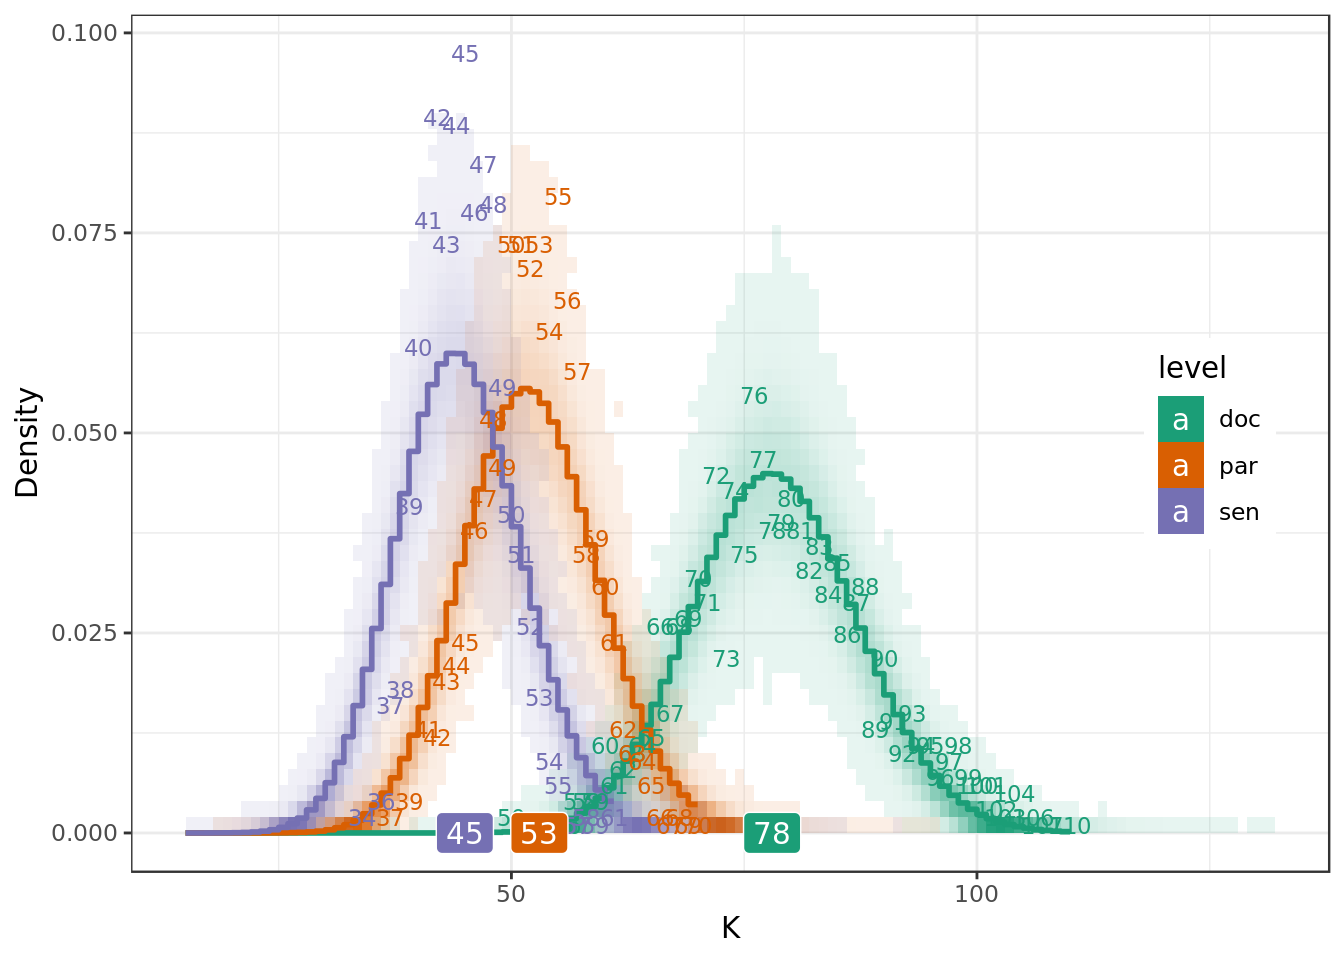
\includegraphics{ambrose_dissertation_files/figure-latex/sim-fig-1} 

}

\caption{Distribution of K by convex hull}\label{fig:sim-fig}
\end{figure}

\begin{table}[!htbp] \centering 
  \caption{Kurtosis Permutation Test} 
  \label{tab:mlk2k} 
\begin{tabular}{@{\extracolsep{5pt}} lrrrrr} 
\\[-1.8ex]\hline 
\hline \\[-1.8ex] 
level & e & se & l99 & u99 & P(e ≦ 0) \\ 
\hline \\[-1.8ex] 
doc & -0.0932 & 0.1149 & -0.3682 & 0.2252 & 0.7948 \\ 
par & -0.1125 & 0.1206 & -0.3999 & 0.2185 & 0.8257 \\ 
sen & 0.0118 & 0.2304 & -0.5078 & 0.6471 & 0.4973 \\ 
\hline \\[-1.8ex] 
\end{tabular} 
\end{table}

\begin{figure}

{\centering 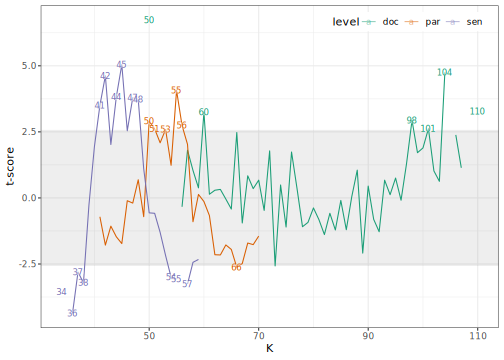
\includegraphics{ambrose_dissertation_files/figure-latex/mlk-tab-1} 

}

\caption{Significant Counts of K}\label{fig:mlk-tab}
\end{figure}

\hypertarget{model-selection}{%
\section{Model selection}\label{model-selection}}

\hypertarget{ten}{%
\chapter{The Development of Intensive Referencing}\label{ten}}

\hypertarget{abstract-4}{%
\subsubsection*{Abstract}\label{abstract-4}}


Early in the history of the U.S. social sciences, scholars
tended to extend the space of references into new territories. After a
transition point in the 1920s, they shifted toward an intensive pattern
of citation where scholars routinely retraced well-trodden steps in the
citation space. The transition coincides with the development of
professional labor markets in the social sciences.

\hypertarget{keywords-4}{%
\subsubsection*{Keywords}\label{keywords-4}}


poisson, permutation test, historical development,
citation, bibliometry, history of social science

\#\#intro

The citation network of scholarship is a critical analytical tool in
bibliometry; indeed the field was revolutionized by the advent of
citation indexing. Nonetheless the concept has alternately been treated
as an analytical device and as a characterization of the phenomenon,
what I will call an ontology. These are very different approaches to
citation networks. As analytical device, citation networks are
instruments by which the researcher uncovers features of scholarship
that were not visible without application of the network. For instance,
a citation network may reveal a cluster indicating the presence of an
invisible college. The invisible college is not itself a citation
network; perhaps it is research partnership may be a local phenomenon
explained by facts on the ground that have little to do with citations.
When treated as an ontology, the researcher reifies the citation network
as the real phenomenon; the network tends to explain itself. An article,
in making a citation, creates a conduit allowing knowledge or influence
to flow into it. It is via the citation that knowledge happens. The
ontology may depend on how the citation network is constructed. In a
knowledge flow network, citations are directed links, and sending and
receiving articles have equal status as nodes. In a co-reference
network, citations are nodes, and articles are links among those
citations appearing in the articles' bibliographies. Because such a
network is undirected there can be no ontology of knowledge flow. The
citation network, however, is an historical development that privileges
the professional aspect of the university. The citation network allows
national and international relations to dominate local ones. It allows
publication to dominate all other venues of intellectual production.

\hypertarget{method-1}{%
\section{method}\label{method-1}}

For every year, find distribution of bibliography size. We will draw
from this to show the effect of variation in bibliography lengths. We
may already surmise that extreme values will create some instability.

For every year, find edge weight distribution, including zeroes.

Find size of total ``space'' in which edes might be laid down. Find
total number of co-citations.

Simulate simple poisson in that space.

Compare to simulation of actually bibliographies in that space.

Test hypothesis that there is a move from extensive to intensive
development.

\hypertarget{lit-review}{%
\section{lit review}\label{lit-review}}

\bibliography{references.bib}


\end{document}
                         % Chapter 1 of dissertation
%\input {chapter2}                         % Chapter 2
%\input {chapter3}                         % etc.
%\input {chapter4}
%\input {chapter5}
%\input {chapter6}
%\input {chapter7}
%\input {chapter8}

\bibliography {references}    % bibliography references
\bibliographystyle {thesis}

\end {document}

